%TeX-design af MatCamp-sanghæftet blev udført af Sune Precht Reeh (SPR)

\documentclass[a4paper,12pt,final,twoside,openany,article]{memoir}%,oneside

\settypeblocksize{0.85\paperheight}{0.9\paperwidth}{*}
%One-sided
%\setlrmargins{*}{*}{1}
%Two-sided
\setlrmargins{*}{*}{.66}

\setulmargins{*}{*}{*}
%\setheadfoot{\onelineskip}{0pt}
\setheadfoot{0pt}{\onelineskip}
\checkandfixthelayout

%\OnehalfSpacing

%\setsecnumdepth{subsection}
%\chapterstyle{tandh}
%\chapterstyle{section}
%\renewcommand{\chaptitlefont}{\bfseries\Large}
%\renewcommand{\chapnumfont}{\bfseries\Large}
\chapterstyle{article}


\usepackage[utf8x]{inputenc}
\usepackage[danish, english]{babel}
\usepackage{amssymb}
\usepackage{stmaryrd}
\usepackage{amsmath}
\usepackage{amsthm}
%\usepackage{eucal}
%\usepackage{subfigure}
\usepackage[pdftex]{color, graphicx}
\usepackage[final]{pdfpages}
\usepackage[final]{hyperref}

\usepackage{tabularx}
\usepackage{multicol}
\setlength{\vleftmargin}{0em}
\setlength{\columnsep}{30pt}
\usepackage[none]{hyphenat}


\usepackage{tikz}
\usepackage{todonotes}

\renewcommand{\chaptermark}[1]{\markboth{\thechapter\quad #1}{\thechapter\quad #1}}
\renewcommand{\sectionmark}[1]{\markright{\thesection\quad #1}}
\renewcommand{\tocmark}{\markboth{\contentsname}{\contentsname}}
\renewcommand{\bibmark}{\markboth{\bibname}{\bibname}}
\renewcommand{\glossarymark}{\markboth{\glossaryname}{\glossaryname}}
\renewcommand{\indexmark}{\markboth{\indexname}{\indexname}}

%\makepagestyle{suneNormal}
%\makeoddhead{suneNormal}{\scshape\rightmark}{}{\bfseries\thepage}
%\makeevenhead{suneNormal}{\bfseries\thepage}{}{\scshape\rightmark}
%\makeheadrule{suneNormal}{\textwidth}{\normalrulethickness}
%\pagestyle{suneNormal}
%\copypagestyle{suneChapter}{suneNormal}
%\makeoddhead{suneChapter}{\scshape\leftmark}{}{\bfseries\thepage}
%\makeevenhead{suneChapter}{\bfseries\thepage}{}{\scshape\leftmark}
%\aliaspagestyle{chapter}{suneChapter}

\makepagestyle{sangbog}
\makeoddfoot{sangbog}{}{}{\large\bfseries\thepage}%\makeoddfoot{sangbog}{}{}{\large\thepage}
\makeevenfoot{sangbog}{\large\bfseries\thepage}{}{}%\makeevenfoot{sangbog}{\large\thepage}{}{}
\copypagestyle{sangbogGreek}{sangbog}
\makeoddfoot{sangbogGreek}{}{}{\large\boldmath\pageAutoShift{\thepage}}%\makeoddfoot{sangbog}{}{}{\large\thepage}
\makeevenfoot{sangbogGreek}{\large\boldmath\pageAutoShift{\thepage}}{}{}%\makeevenfoot{sangbog}{\large\thepage}{}{}

\pagestyle{sangbogGreek}
\aliaspagestyle{chapter}{empty}


\makepagestyle{front}
\makeoddfoot{front}{}{}{\large\bfseries Ungdommens Naturvidenskabelige Forening}
\makeevenfoot{front}{}{}{\large\bfseries Ungdommens Naturvidenskabelige Forening}


\numberwithin{equation}{chapter}
\numberwithin{figure}{chapter}
\numberwithin{table}{chapter}
\frenchspacing

%\makeindex
%\makeglossary

%How the glossary looks
%\changeglossactual{+}
%\changeglossnum{\thepage}
\changeglossnumformat{|hyperpage}%% for hyperlinks

%Ugly hack so \colon survives into the glossary
%\renewcommand*{\begintheglossaryhook}{\newcommand{\colonn}{\colon}}

\newbox\tempboxa
\renewcommand{\glossitem}[4]{%
\sbox\tempboxa{#1 \quad #2 #3 #4}%
\par
\ifdim\wd\tempboxa<0.8\linewidth
#1 \quad #2 #3 \dotfill #4\relax
\else
\hangindent 2em
#1 \dotfill #4\\
#2 #3
%#1 \dotfill #4\\
%\parbox{\linewidth}{
%\leftskip 2em\rightskip 1em
%#2 #3
%}
\fi
}




% New commands
\newcommand{\e}[0]{$\varepsilon$}
\newcommand{\ph}[0]{$\varphi$}

\newcommand{\Z}[0]{\mathbb Z}
\newcommand{\N}[0]{\mathbb N}
\newcommand{\R}[0]{\mathbb R}
\newcommand{\Q}[0]{\mathbb Q}
\newcommand{\C}[0]{\mathbb C}

\newcommand{\lrepeat}{\ensuremath{\lVert : \,}}
\newcommand{\rrepeat}{\ensuremath{\, : \rVert}}


% TikZ for graphs and diagrams
\usetikzlibrary{arrows,matrix}
\tikzset{dot/.style={circle,fill=black,thick,inner sep=0pt,minimum size=1mm,draw}}
\tikzset{arrow/.style={semithick,>=stealth',shorten >=1pt,shorten <=1pt}}
%\tikzset{arrow/.style={semithick,>=to,shorten >=1pt,shorten <=1pt}}
\tikzset{equal/.style={arrow,double distance=2pt}}

%Enumerating with small roman integers as standard
\renewcommand{\theenumi}{(\roman{enumi})}\renewcommand{\labelenumi}{\theenumi}

\makeatletter
\newcommand*{\greek}[1]{%
  \expandafter\@greek\csname c@#1\endcsname
}
\newcommand*{\@greek}[1]{%
  $\ifcase#1
  \or\alpha\or\beta\or\gamma\or\delta\or\varepsilon
  \or\zeta\or\eta\or\theta\or\iota\or\kappa\or\lambda
  \or\mu\or\nu\or\xi\or o\or\pi\or\rho\or\sigma
  \or\tau\or\upsilon\or\varphi\or\chi\or\psi\or\omega
  \or\text{\bfseries \ae}\or\text{\bfseries \o}\or\text{\bfseries \aa}
  \or\mathfrak a\or\mathfrak b\or\mathfrak c\or\mathfrak d\or\mathfrak e
  \else\@ctrerr\fi$
}
\newcommand*{\Greek}[1]{%
  \expandafter\@Greek\csname c@#1\endcsname
}
\newcommand*{\@Greek}[1]{%
  \ifcase#1\or A\or B\or$\Gamma$\or$\Delta$\or E
  \or Z\or H\or$\Theta$\or I\or K\or$\Lambda$
  \or M\or N\or$\Xi$\or O\or$\Pi$\or P\or$\Sigma$
  \or T\or Y\or$\Phi$\or X\or$\Psi$\or$\Omega$
  \or$\mathfrak A$\or$\mathfrak B$\or$\mathfrak C$\or$\mathfrak D$
  \or$\mathfrak E$\or$\mathfrak F$\or$\mathfrak G$\or$\mathfrak H$
  \else\@ctrerr\fi
}

\newcommand*{\symcount}[1]{%
  \expandafter\@symcount\csname c@#1\endcsname
}
\newcommand*{\@symcount}[1]{%
  $\ifcase#1
  1\or2\or3
  \or 4\or 5\or6\or7\or 8\or 9 \or 11\or12\or13
  \or 14\or15\or 16\or17
  \or18
  \or 19\or 20
  \or 21\or 22
  \or 23
  \or24\or25\or 26\or 27
  \or28\or29\or30
  \or31\or32\or33\or34\or35\or36\or37\or38\or39\or40\or41\or42\or43\or44\or45\or46\or47\or48\or49\or50\or51\or52
  \else\@ctrerr\fi$
}

\newcommand*{\intcount}[1]{%
  \expandafter\@intcount\csname c@#1\endcsname
}
\newcommand*{\@intcount}[1]{%
  $\ifcase#1
  1\or2\or3
  \or 4\or 5\or6\or7\or 8\or 9
  \or10 \or 11\or12\or13
  \or 14\or15\or 16\or17
  \or18
  \or 19\or 20
  \or 21\or 22
  \or 23
  \or24\or25\or 26\or 27
  \or28\or29\or30
  \or31\or32\or33\or34\or35\or36\or37\or38\or39\or40\or41\or42\or43\or44\or45\or46\or47\or48\or49\or50\or51\or52
  \else\@ctrerr\fi$
}

\makeatother


\newcommand{\standardpage}{\arabic{page}}
\renewcommand{\thepage}{\standardpage}
\newcommand{\standardpoem}{\arabic{poem}}
\renewcommand{\thepoem}{\standardpoem}
%\setcounter{page}{0}


%Indikerer om Fulbert og Beatrice er passeret - så efterfølgende sidetal skal rykkes:
\newif\ifFulbert

\newcounter{value}
%Til udskrivning af sidetal på de enkelte sider (afhængigt af Fulbert og Beatrice):
\newcommand{\pageAutoShift}[1]{
    \setcounter{value}{#1}
    \ifFulbert
        \addtocounter{value}{-1}
    \fi
    %{\boldmath\greek{value}}
    {\boldmath\symcount{value}}
}
%Til udskrivning af sidetal i indeks (afhængigt af Fulbert og Beatrice):
\newcommand{\pageNoShift}[1]{
    \setcounter{value}{#1}
    %{\boldmath\greek{value}}
    {\boldmath\symcount{value}}
}
\newcommand{\pageWithShift}[1]{
    \setcounter{value}{#1}
    \addtocounter{value}{-1}
    %{\boldmath\greek{value}}
    {\boldmath\symcount{value}}
}

%Opretter sang i indeks - med korrekt sidetal (afhængigt af Fulbert og Beatrice).
%Syntaksen er følgende: \autoIndex[<alfabetisering>]{<sangtitel>}
\newcommand{\autoIndex}[2][]{
\ifthenelse{\equal{#1}{}}
{\autoIndexHelp{#2}{#2}}
{\autoIndexHelp{#1}{#2}}
}
\newcommand{\autoIndexHelp}[2]{
\ifFulbert
\index{#1@\protect\flagverse{\thepoem}#2|pageWithShift}
\else
\index{#1@\protect\flagverse{\thepoem}#2|pageNoShift}
\fi
}
\begin{comment}
\newcommand{\autoIndex}[2][{#2}]{
\ifFulbert
\index{{#1}@\protect\flagverse{\thepoem}{#2}|pageWithShift}
\else
\index{{#1}@\protect\flagverse{\thepoem}{#2}|pageNoShift}
\fi
}
\end{comment}



%\xindyindex
\makeindex
%\makeglossary



\title{Sangbog for Matematik Camp 2013}
\author{Ungdommens Naturvidenskabelige Forening}
\date{\today}


\begin{document}
%\maketitle

\thispagestyle{empty}

\centering

\phantom{test}
\vspace{1cm}

%Den uautoriserede forside
%\mbox{\includegraphics[trim=4cm 10cm 5.5cm 10cm]{matcamp2012.pdf}}

\mbox{
\includegraphics[clip,trim=1cm 10cm 1cm 5cm,scale=.7]{Unflogo.pdf}}

\vspace{1cm}

%{\centering%\fontencoding{T1}
%{\fontfamily{phv}\selectfont\fontsize{2cm}{1em} Matematik\\ Camp 2013}}
%\mbox{\includegraphics[clip,trim=5cm 15cm 15cm 1cm,scale=1.3]{Matematik_Camp_2013.pdf}}
\mbox{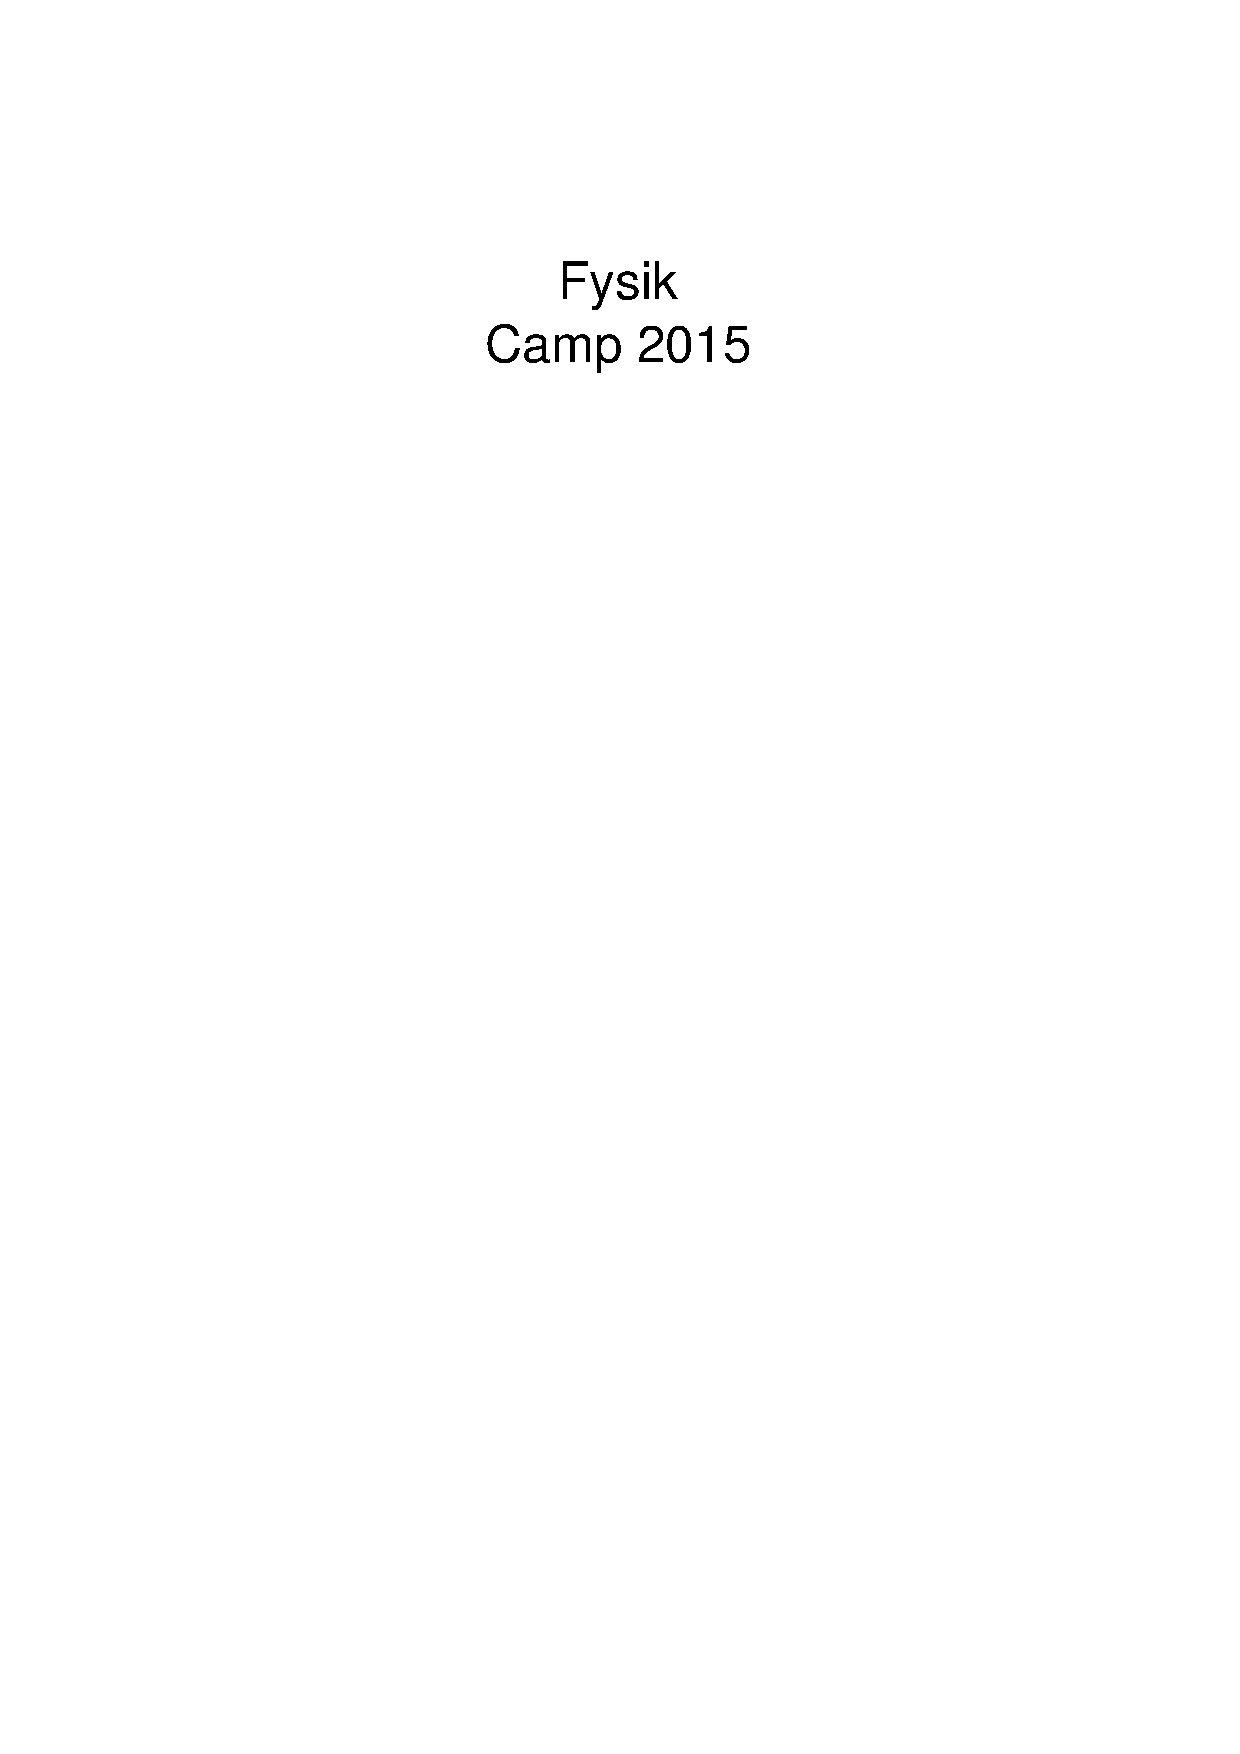
\includegraphics[clip,trim=7cm 23cm 7cm 4cm,scale=2.3]{MatCamp2014_tekst.pdf}}


\vspace{2.5cm}
{\HUGE\bfseries Sanghæfte}

\newpage
\raggedright

%\thispagestyle{empty}
%\phantom.

\newpage
%\setcounter{page}{0}

\NumberPoemTitle
\renewcommand{\PoemTitlefont}{\normalfont\bfseries\large\centering}
\renewcommand{\PoemTitlenumfont}{\normalfont\bfseries\large\centering}
\renewcommand{\afterPoemTitlenum}{\quad}

\PoemTitle{Vi kan ikke li'}\autoIndex[Vi kan ikke li']{Vi kan ikke li'}
\centering{Melodi: Vores buschauffør kan ikke køre bus}\\[.2em]
%\centering{\small\itshape Terese og andre}

{\setlength{\columnsep}{15pt}
\begin{multicols}{3}
\settowidth{\versewidth}{Vi kan ikke li' folk fra matematik\ldots}
\begin{verse}[\versewidth]
Vi kan ikke li' folk
vi ik' kan li'\\
Vi kan ikke li' folk
vi ik' kan li'\\
For vi kan sgu ikke li' dem,\\
de skulle hellere tage at blive hjemme\\
Vi kan ikke li' folk
vi ik' kan li'

Vi kan ikke li' folk fra teologi\ldots\\
For de er nogle hængemuler,\\
tror at helligånden puler

Vi kan ikke li' folk fra biologi\ldots\\
For de går i strikketrøjer,\\
og med dyrene sig fornøjer

Vi kan ikke li' folk der har fysik\ldots\\
For de har sgu nogle testikler\\
der er på størrelse med partikler

Vi kan ikke li' folk fra musikvidenskab\ldots\\
For de er nogle lamme nødder,\\
passer ikke på versefødder

Vi kan ikke li' folk fra nano-tek\ldots\\
De går rundt med sure miner,\\
laver bittesmå maskiner

Vi kan ikke li' folk fra statistik\ldots\\
De vil hypoteser teste\\
mens de hel're burde feste
\columnbreak

Vi kan ikke li' folk fra arkæologi\ldots\\
fordi de graver og de graver\\
og på gamle mennesker rager

Vi kan ikke li' folk fra filosofi\ldots\\
for de går bar' og funderer\\
om de selv mon eksisterer

Vi kan ikke li' folk fra farmaci\ldots\\
for de går og triller piller\\
og tabletter og pastiller

Vi kan ikke li' folk fra geologi\ldots\\
For de går og ser på stenene\\
når de burde sprede benene

Vi kan ikke li' folk fra astronomi\ldots\\
De er fjolser uden hjerner\\
der går rundt og ser på stjerner

%Vi kan ikke li' folk fra iNano\ldots\\
%bagfra blir' de lidt for kække\\
%synes Ångstrøm de er frække

Vi kan ikke li' folk fra økonomi\ldots\\
For de regner på budgettet\\
når de sidder på toilettet

Vi kan ikke li' folk fra lingvistik\ldots\\
Kulli waffli zarka gunku\\
emfle birnan smöja dunku

Vi kan ikke li' folk der har kemi\ldots\\
For de hedder Ion og Ester\\
mens de luften stærkt forpester

Vi kan ikke li' folk fra matematik\ldots\\
For de teoretiserer\\
indtil $2$ plus $3$ bli'r $4$
\columnbreak

Vi kan ikke li' folk der har IT\ldots\\
Uni skaffer studiejobbet\\
Det er næsten alt for snobbet

Vi kan ikke li' folk der har dat-mult\ldots\\
Datalogcirkusartister;\\
de er næsten humanister

%Vi kan ikke li' folk der har tek-fys\ldots\\
%for de har en bærbar PC\\
%læser mails når de' på WC

%Vi kan ikke li' folk fra statskundskab\ldots\\
%for de gider kun at kom' for-\\ di
%de tror de møder Lomborg

%Vi kan ikke li' folk fra farmaceutisk kemi\ldots\\
%de fungerer som en buffer\\
%der i alle emner skuffer

Vi kan ikke li' folk fra medicin\ldots\\
For de går i hvide kitler,\\
og det rimer jo på Hitler

Vi kan ikke li' folk fra molekylær
(biologi)\ldots\\
for de kloner små kaniner\\
splejser dem med appelsiner

Vi kan ikke li' folk fra psykologi\ldots\\
For de vader rundt i læder,\\
og de hader deres fædre

Vi kan ikke li' folk der er jurister\ldots\\
for med hule paragraffer\\
dagen lang sig selv de straffer

Vi kan ikke li' folk der har historie\ldots\\
for de har kun gamle minder\\
og et job de aldrig finder

Vi kan ikke li' folk der har idræt\ldots\\
For de ligner jo rødbeder,\\
når de render rundt og sveder

Vi kan ikke li' folk fra datalogi\ldots
\end{verse}
\end{multicols}
}

\newpage

\PoemTitle{Bobbelsortering}\autoIndex[Bobbelsortering]{Bobbelsortering}
{Melodi:Liva Weel - Lad det boble}\\[.2em]
{\small\itshape DIKUrevy 2013}
\begin{multicols}2
\settowidth{\versewidth}{Når engang jeg bobler helt på plads}
\begin{verse}[\versewidth]

Ret din peger mod dit datasæt\\
følg nu med, lad vær' at blive træt.\\
Algoritmen listen traverserer\\
data vi sorterer ret.

Tag to tal og se på deres værdi\\
er det mindre, bytter vi fordi\\
facit søges, korrekthed øges.\\
Så'n er datalogi.

Lad dem boble, boble, boble,\\
bytte om på de her to\\
blot programmet terminerer,\\
kan jeg sagtens her bestå.

Når man først sit emne trækker\\
og hukommelsen den strejker\\
håber gavmildheden rækker\\
bare manglerne er få.

Jeg behøver aldrig lære fler'\\
hvis jeg kan bevise denne her\\
andre algoritmer de er svære\\
siger vores lærebog.

Når engang jeg bobler helt på plads\\
er al tiden gået er mit sats.\\
Min metode er langsom kod'\\
Pawels spørgsmål gør nas.

Lad dem boble, boble, boble,\\
bytte om på de her to\\
vi kan se det terminerer,\\
ergo pensum jeg forstår.

Når I nu om lidt voterer\\
skal I husk' hvad jeg præsterer:\\
Algoritmen terminerer\\
så lad mig nu bestå!

\end{verse}
\end{multicols}

\PoemTitle{function fib(n)}\autoIndex[function fibn]{function fib(n)}
{Melodi:Sarah Brightman og Andrea Bocelli - Time to say goodbye}\\[.2em]
{\small\itshape DIKUrevy 2009}
\begin{multicols}2
\settowidth{\versewidth}{Læser man på DIKU skal man kunne programmere rekursioner}
\begin{verse}[\versewidth]


Læser man på DIKU skal man kunne programmere rekursioner\\
Man kan gøre det i Matlab kun med ganske få allokationer

Let som en leg\\
Kod med mig, med mig

Tænd for din laptop\\
Slå nu guien fra med \texttt{'matlab -nodesktop'}\\
Vi kan programmer'\\
og kalkuler'\\
Fibonaccis talrække

\texttt{function fib(n)}\\
\hspace*{3mm}\texttt{p = 0;}\\
\hspace*{3mm}\texttt{A = 1}\\
\hspace*{3mm}\texttt{for j = 1 : n}\\
\hspace*{3mm}\hspace*{3mm}\texttt{temp = A;}\\
\hspace*{3mm}\hspace*{3mm}\texttt{A = A + p}\\
\hspace*{3mm}\hspace*{3mm}\texttt{p = temp;}\\
\hspace*{3mm}\texttt{end}

og programmet er slut
\end{verse}
\end{multicols}

\newpage
\PoemTitle{Faster than Light}\autoIndex[Faster than Light]{Faster than Light}
{Melodi:Backstreet Boys - Larger than Life}
{\small\itshape FysikRevy  2012}
\settowidth{\versewidth}{A pretty student comes and she looks so magnificent}
\begin{multicols}2
\begin{verse}[\versewidth]

We are working hard at il OPERA experiment\\
A pretty student comes and she looks so magnificent\\
blonde hair, stilleto, and soft skin so bright

Small neutrinos - hard to see, hard to see\\
we need to determine their velocity\\
(to) concentrate is hard (with) pretty girls in sight\\
And that makes them faster than light

Gorgeous bella donna make us drop our activity\\
Now we have refuted general relativity\\
blonde hair, stilleto, soft skin so bright

Small neutrinos - hard to see, hard to see ...

blonde hair, stilleto, soft skin so bright

Small neutrinos - hard to see, hard to see ...
\end{verse}
\end{multicols}

\PoemTitle{Koder Kapitalen}\autoIndex[Koder Kapitalen]{Koder Kapitalen}
{Melodi:Kim Hot - Smoker Industrien}\\[.2em]
{\small\itshape DIKUrevy 2013}
\begin{multicols}{2}
\settowidth{\versewidth}{man bli'r tævet med klassestil til man ka' Javaetikette.}
\begin{verse}[\versewidth]

For 20 år siden der vidste folk ik'\\
at datalogi det ku' blive så fedt!\\
Der var en mand, der vidste det lidt\\
men han koded' slam og fortalt' det ik\\
men den mand han ku' se, at der kom et sprog\\
hvor alle der koded' ku' ligne et fjog!\\
Det fucking køter sprog det kørt' i en VM\\
og med \texttt{static void main} bli'r det hele så nemt!

Det var 20 år siden og hans navn var Karl Koder\\
koded' slam for kapitalen, havde syge frynsegoder\\
Bawlet i Eclipse og spurgt': "Har du et problem?"\\
Så skal Karl nok kom' og kode dit system.

Der var en konkurrence hvor han ik' sagde slut,\\
for Karl han sgu battle mod motherfucking Knuth!\\
Hans første linjer kode de var ik' særligt dope,\\
men resten de var bomben, for de brugte nemlig SOAP!

Karl vandt og ham Knuth fik piveren på!\\
Tog tilbage til Stanford den BØSSEKAL!\\
Karl han sagde til den anden: "Pas godt på køter Java",\\
for det' fremtidssproget, der bliver fuldstændig fucked,\\
vi skal kode det hele! Forstår du det?\\
Og det skal kodes i Java, der må ik' vær' noget C!\\
Så fuck købsaftalen, tør røv med manualen\\
navnet er Køter Karl, og vi koder kapitalen!

Koder ik i C,\\
heller ej VB,\\
eller det der lodne PHP\\
han koder Java,\\
kongen af Java,\\
han koder altid,\\
alting i Java!

Koder ik i C,\\
heller ej VB,\\
eller det der lodne PHP\\
han koder Java,\\
kongen af Java,\\
kongen af Java,\\
kongen af Java!

Nu står jeg her igen! Mand mod mand\\
Parat til at kod' hvad du ik' kan!\\
For datalogi det er blevet så fedt,\\
man kan lave en service på internet!\\
Og når den bli'r sat op, så kører den på Tomcat\\
og så ta'r Karl hjem, og holder sig en sabbat,\\
og så si'r han til sin chef:\\
"Fuck din kode! Det er UML din BØSSEKAL!"\\
Det skal kodes i Java! Det skal kodes med SOAP\\
I en managed verden uden at tænke på scope.\\
Hvor man elsker Swing, og bli'r fuldstændig fucked,\\
Så længe man koder Java, så går det godt!\\
Så alle de svanser, som der koder det i VB\\
Det skal nok blive godt med nog't Java på jeres CV\\
Så tag hjem fra regn'centralen og kod kapitalen!\\
Fræse lortet ned med SOAP, regulere hele dagen!

Koder ik i C ...\\
Koder ik i C ...

Når nu dikufanter de vil sælge kod' til nogen,\\
kan de lære et par hacks inde på Kongens kodeskole\\
Det første øvel'shold, det hedder SOAP-vold\\
Man bli'r låst inde i Hel, og skal håndkod' XML!\\
Den anden disciplin, den er ik' så nem at gætte,\\
man bli'r tævet med klassestil til man ka' Javaetikette.\\
Den tredje disciplin, det' alt for fedt\\
Du skal kode noget Java for HI-PER-FIT.\\
Man sletter GHC, starter Java-IDE\\
Fucker deres lambda, det en syg idé\\
Man lærer de svanser at hyle som en kat\\
når man breaker deres build hver eneste nat\\
Den allersidste time er lavningsdisciplin,\\
for når du koder Java, så bli'r damerne til dine,\\
Så fuck kvaliteten og skid på omtalen\\
Foran terminalen kan du kode kapitalen!

Koder ik i C ...\\
Koder ik i C ...\\
Koder ik i C ...\\
Koder ik i C ...

Koder Karl...

\end{verse}
\end{multicols}

\PoemTitle{Doktrinen}\autoIndex[Doktrinen]{Doktrinen}
{Melodi:Otto Brandenburg - Alle sømænd er glade for piger}\\[.2em]
{\small\itshape DIKUrevy 2009}
\begin{multicols}2
\settowidth{\versewidth}{Foruden lidt Delphi, og Python og Ruby}
\begin{verse}[\versewidth]

Alle russer skal lære doktrinen\\
man skal kode i Moscow ML\\
men de modsætter sig disciplinen\\
når de sidder bag skærmene selv

Og koder i Java, C\# eller Ada\\
selv Fortran og Matlab, og HTML\\
Foruden lidt Delphi, og Python og Ruby\\
og Visual Basic med MySQL

Som instruktor er ansvaret mit\\
russers uvaner skal rettes ind\\
de skal ik' tro at valget er frit\\
for de lærer jo ikke en pind

Når de koder i Java, C\# eller Ada ...

Efter tolv år er jeg kandidat\\
Kapitalen den kalder på mig\\
min doktrin havde nul resultat\\
for på arbejdet der sidder jeg

Og koder i Java, C\# eller Ada ...
\end{verse}
\end{multicols}
\newpage

\PoemTitle{Ode til bacon}\autoIndex{Ode til bacon}
{Melodi: Backstreet boys -- I want it that way}\\[.2em]
{\small\itshape Rasmus Fruergaard-Pedersen, Julerevy 2005}

\begin{multicols}2
\settowidth{\versewidth}{Du blir hvad du spiser, så blir jeg en gris, ja.}
\begin{verse}[\versewidth]
Gik hen i Fø\TeX.\\
Det var en refleks.\\
Det var med en ræson.\\
Jeg sku’ ha’ bacon.

Jeg så i disken,\\
helt tom. Jeg følte\\
på min vom – var som beton.\\
Den skal ha’ bacon.

\emph{Hvorfor er\\
der tomt i køledisken?\\
Hvorfor er\\
der ingen lækkerbidsken?\\
Og hvor er\\
den gris der’ skåret i facon?\\
Jeg vil ha’ bacon.}

Jeg så i vantro.\\
(Vægt)-vogterne de stod og lo.\\
Kom nu herhen smag vor karton.\\
Nej, jeg vil ha’ bacon.

\emph{Hvorfor er\\
der tomt i køledisken?\\
Hvorfor er\\
der ingen lækkerbidsken?\\
Og hvor er\\
den gris der’ skåret i facon?\\
Jeg vil ha’ bacon.}
\columnbreak

Smagen kan give dig lysten til livet,\\
selvom du er vegetar, Aaah!\\
Du blir hvad du spiser, så blir jeg en gris, ja.\\
Det’ hel’re end hundred’ år!

Stegt let med smør til.\\
Svøbt om pølser på grill.\\
Stegt sprødt,\\
stegt sprødt, stegt sprødt, stegt sprødt\ldots\\
Svøb flæsk i bacon!

Stegt i smør eller helt naturel.\\
Føler mig så høj og kulturel.\\
Jeg ku’ synge ud fra en balkon:\\
``Jeg vil ha’ bacon.''

\emph{Smag på lidt\\
bacon svøbt om dejlig mørksej.\\
Smag på lidt\\
bacon fyldt i julepostej.\\
Smag på lidt\\
bacon strøget let med stærk dijon, dijon.\\
Smag på lidt bacon.}

\emph{Giv mig en\\
bacon-krydder-frikadelle.\\
Jeg har lyst\\
til en saltet stegt fedtcelle.\\
Hvem laver\\
mig en saltet flæskesværs-bonbon?\\
Jeg hylder bacon.\\
For jeg vil ha’ baco-o-o-n-n-n-n.}
\end{verse}
\end{multicols}

\newpage

\PoemTitle{Server'n er Crashed}\autoIndex[Server'n er Crashed]{Server'n er Crashed}
{Melodi:Backstreet Boys - I Want It That Way}\\[.2em]
{\small\itshape DIKUrevy 2011}
\begin{multicols}3
\settowidth{\versewidth}{Jeg burde ha' tjekket, men surfede porn}
\begin{verse}[\versewidth]

Yeah!\\
Jeg bli'r\\
helt ked, men\\
Nu er\\
den nede\\
Den var belastet\\
Nu er den crashed.

Min prompt\\
den sejler.\\
System-\\
et fejler\\
Der er sgu knas med\\
den server, der crashed.

For åh nej.\\
Vi sku' ha købt et nyt raid\\
For åh nej\\
Jeg var sgu' ikke beredt.\\
før vi så\\
undtagelsen den kasted.\\
Server'n er crashed

Men kan\\
den tvinges\\
til at\\
ku' pinges\\
Nej, den er - helt trashed\\
ja, server'n er crashed.

For åh nej ...

Tænkte, jeg fikser det bare i mor'n\\
da den stod der og kasted' fejl\\
yeah\\
Jeg burde ha' tjekket, men surfede porn\\
Nu er den sgu' gåe't sin vej.

Det' ikk'\\
så skid' rart\\
Jeg ta'r\\
en genstart\\
Men nej\\
åh nej\\
åh nej\\
åh nej\\
Det fucking neder'n!

Den fejler nu ved startup\\
Vi har sgu ingen backup\\
Disken er sikkert kvæstet\\
Server'n er crashed

For åh nej ...\\
For åh nej ...


Server'n er crashed

\end{verse}
\end{multicols}

\PoemTitle{Lad det gro}\autoIndex[Lad det gro]{Lad det gro}
{Melodi:Frozen - Let It Go}\\[.2em]
{\small\itshape DIKUrevy 2014}
\begin{multicols}3
\settowidth{\versewidth}{Kantinen er tom, der er ingen at se}
\begin{verse}[\versewidth]

Kantinen er tom, der er ingen at se\\
Og jeg drømmer for mig selv\\
Mit ønske er helt umuligt, (men) jeg har håb a-lligevel


Men det vil ik' gro

Det er det alle mennesker vil sig'\\
Gi' mig et skæg!

Lad det gro\\
Kan ik' holde det hem'ligt mer'\\
Lad det gro\\
Det' på hagen det hele sker\\
Lad dem bare glo

Alt det din krop ik' må\\
Alt det jeg ik' kan få

Men i mit ho'ed er en idé\\
Det bli'r fantastisk, prøv at se\\
En datalog kan jeg nu bli'\\
Endelig

Lad det gro\\
Lad det gro\\
Lad dem bare glo


Mit skæg det snor sig som en slange mod mit bryst\\
De tykke lokker hvirvler sig i smukke cirklers lyst\\
Ved Nørrebros Runddel ligger min lykkens borg\\
Det' Fest og Farver, der har reddet os fra sorg

Lad det gro\\
Lad det gro\\
Lad dem bare glo\\
Uden skæg er en datalogs dage talt'
\end{verse}
\end{multicols}
\newpage

\PoemTitle{Spas i Waders}\autoIndex[Spas i Waders]{Spas i Waders}
{Melodi:Hit'n'Hide - Space Invaders}\\[.2em]
{\small\itshape Biorevy 2012}
\begin{multicols}{2}
\settowidth{\versewidth}{Ude i søerne, der har jeg net med småfisk i}
\begin{verse}[\versewidth]

Spas i waders i en så\\
Fanger Myggelarver, Super biolog\\
Spas I waders I en så\\
Se på makrofytter, mål pH og lys

Må afsted, kom nu med

Du er feltbiolog med super seje waders på\\
Render og ta'r prøver dagen lang\\
Jeg er feltbiolog med super seje waders på\\
Renser danske søer for plankton

Spas i waders i en sø ...

Spas i waders i en sø...

Må afsted, kom nu med

Du er feltbiolog udstyret med planktonnet\\
Tæller og nøgler fisk og zooplankton\\
Ude i søerne, der har jeg net med småfisk i\\
At nøgle og måle, det kan jeg li'

Spas i waders i en sø ...

Spas i waders i en sø ...

Du ta'r afsted op til Hillerød\\
Jeg vil med, se på livet i søen\\
 -- Vi finder en ny plankton art\\
Du og jeg tilsammen kan vi alt\\
 -- Vi kan alt

Spas i waders i en sø ...

Spas i waders i en sø ...

Kom nu med!
\end{verse}
\end{multicols}

\PoemTitle{Fag Facisme}\autoIndex[Fag Facisme]{Fag Facisme}
{Melodi:Julia Ward Howe - The Battle Hymn of the Republic}\\[.2em]
{\small\itshape FysikRevy  2013}
\begin{multicols}{2}
\settowidth{\versewidth}{Vi diff'rentierer step-funktioner uden megt' besvær}
\begin{verse}[\versewidth]

Så tak os for at masse faktisk oss' er energi\\
og tak os for konstant forøgelse af entropi\\
og tak os for at tyngdekraften virker overalt\\
for vi følger Newtons kald

Mat'matik approksimeres\\
Datalogen ignoreres\\
Humanister likvideres\\
Ren Fysik det bli'r vor svar!

Så tak os for at verd'nen er en superposition\\
og tak os for at elektronen er en fermion\\
og tak os for at kvantemekanik er mer' end ord\\
Udtænkt af vor Niels Bohr

Mat'matik approksimeres ...

Vi diff'rentierer step-funktioner uden megt' besvær\\
Vi indekserer kun med 1 og nester for-loops her\\
På KUA har I kommunister, dræn og meta-vrøvl\\
Kom an, vi gir' jer høvl

Mat'matik approksimeres ...

Så tak os for at alting overhoved' eksister',\\
og tak os for de svære ting vi dagligt integrer'.\\
Og tak os for at sætte flotte streger gennem $h$\\
ren fysik det vil bestå

Mat'matik approksimeres ...

Mat'matik approksimeres ...
\end{verse}
\end{multicols}
\newpage

\renewcommand{\thepage}{10}
\thispagestyle{sangbog}
\renewcommand{\thepoem}{12}

\newcommand{\boldpage}[1]{{ \boldmath$#1$}}
\PoemTitle{Fulbert og Beatrice}\index{Fulbert og Beatrice@\protect\flagverse{12}Fulbert og Beatrice|boldpage}
{Melodi: En vår er kommet (Jeg plukker fløjlsgræs)}\\[.2em]
%{\small\itshape MatematikRevy 2008}

\begin{multicols}{2}
\settowidth{\versewidth}{Men langvejs drog han en årle morgen,}
\begin{verse}[\versewidth]
I frankens rige, hvor floder rinde\\
som sølverstrømme i lune dal,\\
lå ridderborgen på bjergets tinde\\
med slanke tårne og gylden sal.\\
Og det var sommer med blomsterbrise\\
og suk af elskov i urtegård.\\
Og det var Fulbert og Beatrice,\\
og Beatrice var sytten år.

De havde leget som børn på borgen,\\
mens Fulbert endnu var gangerpilt.\\
Men langvejs drog han en årle morgen,\\
mod Saracenen han higed' vildt.\\
Han spidded' tyrker som pattegrise,\\
et tusind stykker blev lagt på bår,\\
for Fulbert kæmped' for Beatrice,\\
og Beatrice var sytten år.

Med gluttens farver på sølversaddel\\
han havde stridt ved Jerusalem.\\
Han kæmped' kækt uden frygt og dadel\\
og gik til fods hele vejen hjem.\\
Nu sad han atter på bænkens flise\\
og viste stolt sine heltesår,\\
som ganske henrykked' Beatrice\\
for Beatrice var sytten år.

En kappe prydet med små opaler\\
og smagfuldt ternet med tyrkens blod,\\
en ring af guld og et par sandaler\\
den ridder lagde for pigens fod.\\
Og da hun øjnede hans caprise\\
blev hjertet mygt i den væne mår.\\
Af lykke dånede Beatrice,\\
for Beatrice var sytten år.

\columnbreak
Da banked' blodet i heltens tinding,\\
thi ingen helte er gjort af træ.\\
Til trods for plastre og knæforbinding\\
sank ridder Fulbert med stil på knæ.\\
Han kvad: ``Skønjomfru, oh skænk mig lise,\\
thi du alene mit hjerte rår!''\\
``Min helt, min ridder,'' kvad Beatrice,\\
for Beatrice var sytten år.

Og der blev bryllup i højen sale\\
med guldpokaler og troubadour,\\
og under sange og djærven tale\\
blev Fulbert ført til sin jomfrus bur.\\
Og følget hvisked' om øm kurtice\\
og skæmtsom puslen blandt dun og vår.\\
For det var Fulbert og Beatrice,\\
og Beatrice var sytten år.

Men ridder Fulbert den samme aften\\
af borgens sale blev båren død.\\
Den megen krig havde tær't på kraften,\\
og sejrens palmer den sidste brød.\\
Oh bejler, lær da af denne vise:\\
Ød ej din kraft under krigens kår.\\
Nej, spar potensen til Beatrice,\\
når Beatrice er sytten år.
\end{verse}
\end{multicols}

\renewcommand{\thepoem}{\standardpoem}

\newpage
\renewcommand{\thepage}{\standardpage}

%If the later page numbers should be shifted by one, use \Fulberttrue.
\Fulberttrue

\PoemTitle{diff}\autoIndex[diff]{diff}
{Melodi:Aqua - Doctor Jones}\\[.2em]
{\small\itshape DIKUrevy 2013}
\begin{multicols}3
\settowidth{\versewidth}{R: Hey baby, hva' mangler du}
\begin{verse}[\versewidth]

Ofte er filerne ens\\
Lige nu er de det ikke\\
Hvem har mon rørt min C-fil?\\
Hvad har de indsat i koden?

\texttt{void public static}\\
\texttt{void main}, wat?\\
\texttt{void abstract class}, øv!

Men min kode er stor,\\
den kan jeg ikk' oversku'\\
Mangler den rigtige mand,\\
en som kan redde mig nu\\

R: Hey baby, hva' mangler du\\
S: At finde forskelle\\
R: Ska' det være lige nu?\\
S: Kom nu og \texttt{diff}\\
R: Jeg kigger på din' filer nu\\
S: Hva' sker der når du ser?\\
R: Jeg kan nu ingen forskel se, pyt, det kan jo ske

René Diff, Diff,\\
Tjekker filerne.\\
René Diff, René Diff,\\
Er de ens!\\
De er ens!

René Diff, Diff,\\
filernes sherif.\\
René Diff, René Diff,\\
Er de ens!\\
De er ens!

\texttt{void public static} ...

\texttt{void public static} ...

Er der klasser i C?\\
Nej, det er da vist i Java\\
René, kan du ikk' se?\\
Du er et levn fra halvfemserne

R: Hey baby, hva' er det nu\\
S: Dig kan jeg ikke brug'\\
R: Lad mig tjekke den her, du\\
S: Det er en \texttt{.gif}!\\
R: (host) det er et billed' af en grif\\
S: Du var min diff-kalif!\\
R: Hvad vil' du gøre uden mig, jeg er da for sej

René Diff, Diff,\\
lad mig gi' et fif\\
René Diff, René Diff,\\
Styrtflyver!\\
Du lyver!

René Diff, Diff,\\
synger næste riff\\
René Diff, René Diff,\\
Hvad vil du!\\
Ha' ret nu!

\texttt{void public static} ...

\texttt{void public static} ...

Brug'r nu diff3\\
Brug'r nu diff3\\
Brug'r nu diff3\\
Brug'r nu diff3

René Diff, Diff,\\
vågn op nu\\
René Diff, Diff,\\
forstå nu\\
René Diff, Diff,\\
du er sgu\\
René Diff, Diff,\\
i udu

\texttt{void public static} ...

\texttt{void public static} ...

René Diff, Diff\\
Giv min fil et snif\\
René Diff, René Diff\\
Han tog fejl\\
Det gjor' jeg

René Diff, Diff\\
Bruger sans serif\\
René Diff, René Diff\\
Farvel nu!\\
Nå øv du
\end{verse}
\end{multicols}
\newpage

\PoemTitle{Humanist}\autoIndex[Humanist]{Humanist}
{Melodi:Dario von Slutty - Onani}\\[.2em]
{\small\itshape DIKUrevy 2013}
\begin{multicols}1
\settowidth{\versewidth}{men jeg vil bar' være færdig - arbejdsløshed er på mode!}
\begin{verse}[\versewidth]

Humanist - en KUAist\\
Humanist - en KUAist\\
Humanist - det' godt nok trist:\\
Det ta'r dem 10 semestre\\
og kan ikke brug's til sidst.

Nu skal I hør':\\
Jeg er ham der Klaes, jeg har ECTS-behov,\\
men kurserne jeg tager, de gi'r mig aldrig lov.\\
De taler mig i søvne, her til forelæsningen\\
Og når den så er ovre, har jeg det hele glemt igen.

Hvorfor tage kurser, der altid dumper mig?\\
Det er derfor, at jeg siger: "Der er en nem're vej!"

Humanist - en KUAist ...

Humanist - en KUAist ...

Se, de fleste går og drømmer om at arbejde med kode,\\
men jeg vil bar' være færdig - arbejdsløshed er på mode!\\
Jeg er ligeglad med penge, jeg har børneopsparing\\
Og når den så løber tør, kan jeg pizza udbring'.\\
Hvorfor skulle arbejd', og ikke ha' tid til leg?\\
Det er derfor, at jeg siger: "Der er en nem're vej"

Humanist - en KUAist ...

Humanist - en KUAist ...

Nu er det ovre, jeg er endelig blevet fri\\
Er blevet kandidat i østrigsk eskimologi\\
Der findes intet job hvori denne grad kan bruges\\
Så alle jobsamtaler sluttes af med at der buh'es.

Her er det så, jeg fortryder jeg droppede ud\\
Hvis bare jeg kunne kode, så fremtiden lysere ud

Humanist - en KUAist ...

Humanist - en KUAist ...

Datalog - han er jo god\\
Datalog - han er jo god\\
Datalog - får job, værsgo'\\
Det ta'r dem 20 semestre\\
men i det mindste kan de kode.

Datalog - han er jo god ...

Det ta'r dem 20 semestre\\
men i det mindste kan de kode.
\end{verse}
\end{multicols}
\newpage

\PoemTitle{Drop Nu Ud}\autoIndex[Drop Nu Ud]{Drop Nu Ud}
{Melodi:The Lion King - Be Prepared}\\[.2em]
{\small\itshape FysikRevy 2011}
\begin{multicols}{2}
\settowidth{\versewidth}{Jeg udrydder tumper, så studiet skrumper}
\begin{verse}[\versewidth]

I ved at jeg er nederdrægtig\\
Jeg er ond som en anden dekan\\
Ja, min sjæl er der noget fordækt i\\
Men hør nu min udsøgte plan

Med mindre du er overlegen\\
Hvis ikke du er et geni\\
Er det bedst at du skaffes af vejen\\
Og se her har jeg en strategi:

Drop ud - hvis du ikke kan kvante\\
Hvis din IQ er under en-treds\\
Jeg udrydder tumper, så studiet skrumper\\
(Og hvad hvis jeg dumper?)\\
Jeg flår dig i stumper!\\
Hvis du er uværdig og aldrig bli'r færdig\\
Vil jeg knuse dit mod fra dag et\\
Og kun du, lille rus, står for skud\\
Drop nu ud!

(Hah! Hvorfor skulle vi droppe ud? Vi er da helt vildt skarpe)\\
I vil måske forsøge jer med et eksamensspørgsmål her og nu?\\
(Bare kom an Mogens!)\\
Nuvel. Udregn energierne for en partikel i en brønd.\\
(Hurra! Vi bruger bare Newtons love!)\\
(Jaaa! Newton, Newton, la lalalalala!)\\
IDIOTER! I kan ikke løse det uden Schrödingerligningen.\\
(Jamen - det er jo vanvid?)\\
Vanvid?\\
DET. ER. KVANT!!!

(Argh! Skynd jer at lære kvant! Ellers får vi aldrig nogle ECTS!)\\
(ECTS!)\\
(ECTS!!)

(Nu terper vi kvant hele dagen)\\
(Og natten går med QCD.)

Og sku I få lyst til at klage\\
er der intet at gøre ved det.

For søger du inspirationen\\
så siger jeg 'the cake is a lie'\\
Men mangler du motivationen,\\
Så husk blot at 'terpen macht frei!'

Så drop ud - hvis du gerne vil skånes\\
Drop ud, hvis du har livet kært.\\
For her ruller hoveder - bag tonede ruder (Terp nu kvant, terp nu kvant)\\
Du trygler 'vær nådig' - der runger af gråd i (Terp nu kvant, terp nu)\\
eksamenslokalet, din død bliver forhalet\\
og spør' du til din karakter\\
vil jeg ridse 00 i din hud\\
-Drop nu ud!

-Så giv op, fald på knæ, rus, og tud\\
-Drop nu ud!\\
(Mwuhuhahahah!)
\end{verse}
\end{multicols}
\newpage

\PoemTitle{Linieskriverdriversangen}\autoIndex[Linieskriverdriversangen]{Linieskriverdriversangen}
{Melodi:Dyrene i Hakkebakkeskoven "Peberkagebagesangen"}\\[.2em]
{\small\itshape DIKUrevy 2005}
\begin{multicols}3
\settowidth{\versewidth}{men bar' fordi Microsoft de skriver}
\begin{verse}[\versewidth]

Når en skriverdriverskriver\\
skriver linieskriverdriver\\
skal en skriverdriver skrive\\
linieskriverdrivprogram.

For det hedder ikke driver\\
nej, det' bare nog't man skriver\\
men bar' fordi Microsoft de skriver\\
driver bliver driver ikke nødvendigvis korrekt, vel?

Hvis en lagerlærer lærer\\
andre lagerlærer's lære\\
bør der's lagerlærdom lagres\\
i et lærelagerlag.

Men det er jo så'n med lærer\\
at de ik' ka' lagre lære\\
for de kager rundt og tager\\
jo slet ikke hinanden alvorligt, vel?

Når processor'n processerer\\
og processerne bli'r flere\\
og professor'n ik' ka' 'pere\\
fler' processer i hans RAM.

{colb}
Ja, så må vi allokere\\
fler' studerende med mere\\
lager end der's lagerlærer\\
har i lagerlærerlag.

Ja, så må vi allokere\\
fler' studerende med mere\\
tid til at studere negre\\
så de ka' forny mit professorat! Ikke sandt?

Når din vektorlektor nægter\\
at en sektorvektorhægter\\
peger på en sektorvektor\\
er din vektorlektor gal.

For en sektorvektorhægter\\
hægter kun til sektorvekt're\\
og det' nytter ik' at lektor\\
nægter hægters eksistens.

For en sektorvektorhægter\\
hægter kun til sektorvekt're\\
selvom alle vor's indtægter\\
mistes når en vektorlektor møder vektorlektorinspektoren, ikke?

Hvis din pegerpeger peger\\
På noget andet end en peger\\
Så' din pegerpegers pegning\\
Gået hen og blevet gal

For en pegerpeger plejer\\
Kun at peg' på andre peger\\
Så vi retter pegerpeger'n\\
For at den kan bli' normal
\end{verse}
\end{multicols}

\PoemTitle{Minken Mink}\autoIndex{Minken Mink}
{Melodi:Bjørnen Bjørn er en bjørn}\\[.2em]
{\small\itshape Computer Science Camp 2015}
\begin{multicols}2
\settowidth{\versewidth}{Med disse ord skal sandhed skrives (Sandhed skrives)}
\begin{verse}[\versewidth]
Minken Mink er en mink.\\
Minken Mink er en mink.\\
Og den kan li' de fleste, den er så flink,\\
For Minken Mink er en mink

Nogen tror at Minken er en ræv.\\
Nogen tror at Minken er en husmår.\\
Nogen tror at Minken er en kat.\\
Men Minken Mink er en mink.\\
Ja Minken Mink er en mink!

Minken Mink er en mink.\\
Minken Mink er en mink.\\
Og den kan li' arrangører for de er pink\\
For Minken Mink er en mink

Nogen tror at Minken er en ræv.\\
Nogen tror at Minken er en husmår.\\
Nogen tror at Minken er en kat.\\
Men Minken Mink er en mink.\\
Ja Minken Mink er en mink!

\end{verse}
\end{multicols}

\newpage



\PoemTitle{Q.E.D.}\autoIndex[Q.E.D]{Q.E.D}
{Melodi:Within Temptation - Our Solemn Hour}\\[.2em]
{\small\itshape FysikRevy  2010}
\begin{multicols}{2}
\settowidth{\versewidth}{Med disse ord skal sandhed skrives (Sandhed skrives)}
\begin{verse}[\versewidth]

Quod erat demonstrandum!\\
Med disse ord skal sandhed skrives\\
Quod erat demonstrandum!\\
Uvidenheden må fordrives

Quod erat demonstrandum!\\
Quod erat demonstrandum!\\
Quod erat demonstrandum!

Mørket samler sig\\
selv i den mindste krog\\
er logik og logos på tilbagetog\\
Intelligent design\\
og anden overtro\\
videnskaben taber til en astrolog

Så vi må handle snart før det er forbi\\
Slut med tavshed nu det tid at si'e

Quod erat demonstrandum!\\
Med disse ord skal sandhed skrives\\
Quod erat demonstrandum!\\
Uvidenheden må fordrives\\
Quod erat demonstrandum!\\
Skal verden vindes må vi st den bi\\
Naturvidenskabs logik vil gør' dig fri!

En ungdomsgeneration\\
's fornuft sat på auktion\\
Vor fremtid smides bort\\
Vor viden kom til kort\\
Fra Unge Mødre og\\
til Paradise Hotel\\
vores hjerneceller keder sig ihjel

Idiotiens lænker har holdt dig ned'\\
så kom ind i kampen og syng med!

Quod erat demonstrandum! Med disse ord ...

Quod erat demonstrandum! Med disse ord ...

Quod erat demonstrandum! Med disse ord ...

Quod erat demonstrandum!\\
Med disse ord skal sandhed skrives (Sandhed skrives)\\
Quod erat demonstrandum!\\
Uvidenheden må fordrives (må fordrives)\\
Quod erat demonstrandum!\\
Skal verden vindes må vi stå den bi\\
Naturvidenskabs logik vil går' dig fri!
\end{verse}
\end{multicols}
\newpage


\PoemTitle{Koder Hele Natten}\autoIndex[Koder Hele Natten]{Koder Hele Natten}
{Melodi:Rage Against The Machine - Killing In The Name Of}\\[.2em]
{\small\itshape DIKUrevy 2011}
\begin{multicols}{2}
\settowidth{\versewidth}{De bruger magt, til at fjerne vores kantine.}
\begin{verse}[\versewidth]

De bruger magt, til at rykke os til HCØ.\\
De bruger magt, til at fjerne vores kantine.\\
De bruger magt, til at fjerne vores rusture.\\
Nu er det nok, vi sætter hårdt mod hårdt\\
Vi er anonyme, vi er DIKU!

Koder hele natten!

Der er dem der koder VB, det er dem uden et CV\\
Der er dem der koder Brainfuck, de kan ikke få det hårdt nok\\
Der er dem der koder Java, det' det en'ste de kan lave.\\
Der er dem der koder ML, det er os der gør det hel' selv!\\
Kod!

Koder hele natten!\\
Koder hele natten!

I skærmens lys vi skal kode\\
Vi skal besejre hvor klode\\
Ved DIKU danner vi pagten\\
Med cyberkrig får vi magten\\
I skærmens lys vi skal kode\\
Vi skal besejre hvor klode\\
Ved DIKU danner vi pagten\\
Med cyberkrig får vi magten\\
I skærmens lys vi skal kode\\
Vi skal besejre hvor klode\\
Ved DIKU danner vi pagten\\
Med cyberkrig får vi magten!

Rejs jer op, tøm jeres kop, i fællesskab får vi DIKU op!\\
For all' skal vid', med dataslid, vi genvinder nu DIKUs storhedstid!\\
Rejs jer op, tøm jeres kop, i fællesskab får vi DIKU op!\\
For all' skal vid', med dataslid, vi genvinder nu DIKUs storhedstid!

Der er dem der koder VB, det er dem uden et CV ...

Koder hele natten!\\
Koder hele natten!

I skærmens lys vi skal kode\\
Vi skal besejre hvor klode\\
Ved DIKU danner vi pagten\\
Med cyberkrig får vi magten\\
I skærmens lys vi skal kode (hver en bit vi vil se)\\
Vi skal besejre hvor klode (bestem' alt der skal ske)\\
Ved DIKU danner vi pagten (datalog'r når' de størst)\\
Med cyberkrig får vi magten (nettet slukker hvor tørst)\\
I skærmens lys vi skal kode (hver en bit vi vil se)\\
Vi skal besejre hvor klode (bestem' alt der skal ske)\\
Ved DIKU danner vi pagten (datalog'r når' de størst)\\
Med cyberkrig får vi magten

Rejs jer op, tøm jeres kop, i fællesskab får vi DIKU op!\\
For all' skal vid', med dataslid, vi genvinder nu DIKUs storhedstid!\\
Rejs jer op, tøm jeres kop, i fællesskab får vi DIKU op!\\
For all' skal vid', med dataslid, vi genvinder nu DIKUs storhedstid!\\
Kod nu!

Kod! Kod nu!

DIKU, det er nu de skal lære\\
DIKU, vi vil kæmp' for din ære!\\
DIKU, det er nu de skal lære\\
DIKU, vi vil kæmp' for din ære!\\
Hack dem, det er nu i skal kode\\
Hack dem, vi besejrer vor klode\\
Hack dem, det er nu i skal kode\\
Hack dem, vi besejrer vor klode\\
Moderkoder!\\
Kod!
\end{verse}
\end{multicols}
\newpage



\PoemTitle{Jeg vil læse *}\autoIndex[Jeg vil læse *]{Jeg vil læse *}
{Melodi:Regnvejrsdag i november}\\[.2em]
{\small\itshape DIKUrevy 2008}
\begin{multicols}3
\settowidth{\versewidth}{[C]jeg bli'r nok en [Am]stor professor}
\begin{verse}[\versewidth]

Jeg vil læse retorik\\
for jeg fatter ik' en brik\\
jeg vil lær' om sprogfinesser\\
og gå op i petitesser\\
jeg bli'r nok en stor professor\\
jeg vil læse retorik

Jeg vil være teolog\\
selvom lønnen ik' er god\\
tro på gud det er det sande\\
også når man træder vande\\
missionére i fjerne lande\\
jeg vil være teolog

Jeg vil læse medicin\\
tjene penge som et svin\\
jeg vil skær i døde men'sker\\
men jeg er jo også svensker\\
klæde mig i \LaTeX handsker\\
jeg vil læse medicin


Jeg vil læse på kemi\\
hårde stoffer kan jeg li'\\
jeg er skæv fra ni til sytten\\
finsprit hælder jeg i bøtten\\
så jeg ender nok på støtten\\
jeg vil læse på kemi


Jeg vil læse cand.polit\\
for mit men'skesyn er skidt\\
jeg vil skær på hospitaler\\
og på skoler uden kvaler\\
mens jeg holder falske taler\\
jeg vil læse cand.polit


Jeg vil læse på fysik\\
lære kvantemekanik\\
jeg går op Einsteins tanker\\
og jeg er en rigtig dranker\\
kæler for mit fadølsanker\\
Jeg vil læse på fysik


Jeg vil være officér\\
i den danske dronnings hær\\
jeg vil skyde talibaner\\
vifte med de danske faner\\
sprede død i lange baner\\
jeg vil være officér


Historie er mit liv\\
støver rundt i et arkiv\\
Læser i de gamle skrifter\\
selvom jeg får mange rifter\\
Jeg ved alt om Neros drifter\\
For historie er mit liv


Jeg vil være pædagog\\
rende rundt i maosko\\
hjælpe børn i overtøjet\\
så de ikke bli'r tilmøjet\\
du kan tro de er fornøjet\\
jeg vil være pædagog


Jeg vil være aktuar\\
hvor min skæbne den er klar\\
Forsikringsvidenskab er sagen\\
jeg vil ta' en bid af kagen\\
Mens jeg sylter kundeklagen\\
Jeg vil være aktuar

Jeg vil muge ud hos køer\\
køre rundt med trillebør\\
sidde i en kæmpe traktor\\
moms det er en ukendt faktor\\
nu skal grisen ned til slagter\\
jeg vil muge ud hos køer


Jeg vil læse på MI\\
for musik kan alle li'\\
Selvom jeg var sidst i klassen\\
Kan jeg stadig score kassen\\
blot jeg lær' at spille bassen\\
Men jeg kan ikke holde takten

Jeg vil læse æstetik\\
i dansenes mystik\\
Svanens død den kan jeg lide\\
skønt jeg ej er en sylfide\\
vil jeg over scenen glide\\
Jeg vil læse æstetik

Jeg vil læse nano tech\\
for min hjerne drak jeg væk\\
sidte fredag på Caféen?\\
da jeg rigtig sku' gå te'n\\
og jeg vælted om i sneen\\
jeg vil læse nano tech


Jeg vil være datalog\\
og min fremtid den er god\\
gcc det er en gave\\
jeg blir nok en kodeslave\\
jeg vil gerne prøv' at snave\\
jeg vil være datalog
\end{verse}
\end{multicols}
\newpage

\PoemTitle{Jobsøgning}\autoIndex[Jobsøgning]{Jobsøgning}
{Melodi:Klokkeren fra Notre Dame - Hell fire}\\[.2em]
{\small\itshape DIKUrevy 2013}
\begin{multicols}3
\settowidth{\versewidth}{Hvorfor har jeg intet job,}
\begin{verse}[\versewidth]

Hør her, kære venner,\\
I ved at jeg er helt speciel,\\
I ved at jeg aldrig koder slam


Hør her, kære venner,\\
I ved at jeg er bedre end


Så sig mig nu, venner,\\
Hvorfor har jeg intet job,\\
Når underkoderne bli'r revet væk?

Vi ved det ikke!

Hvornår vil de lære

Så kom og kod for ooos!

Med Haskell\\
Og Erlang\\
Bliver jeg overset\\
De job jeg\\
Begærer\\
Bli'r aldrig mig til del...



Det ik' min fejl!

Vi har kaffe!

Det' kapitalens valg af sprog\\
der gør det svært!

  frem.

Du kan også få pizza!

Det' ikk min skyld,

Hvad med bacon?

Hvis kapital'n

Eller kage?

Går konkurs fordi de sagde nej til mig!

Sig nu ja, vi vil ha' dig!

Hvorfor skal man bare\\
Acceptere dårlig stil,\\
Finde sig i BlueJ og Eclipse?

Og ofre sin sjæl på\\
Javas alter for et job?\\
Jeg vil aldrig kode OOP!

Med ALGOL\\
Og Agda\\
Holder jeg mig obskur.\\
De fanger\\
Mig aldrig\\
Undslipper gang på gang!

Vi giver snart helt op.

Hvis de vidste besked...

Vil du have det job?

Hvis de bare indså...

Han får aldrig et job.


Jeg kan ikke kode\\
NOGET\\
SOM\\
HEEEELST!
\end{verse}
\end{multicols}
\newpage

\PoemTitle{Facebookevents}\autoIndex[Facebookevents]{Facebookevents}
{Melodi:TV2 - Det Mørke Jylland}\\[.2em]
{\small\itshape DIKUrevy 2014}
\begin{multicols}{2}
\settowidth{\versewidth}{Jeg ved at jeg sandsynligvis går glip af noget}
\begin{verse}[\versewidth]

Jeg tjekker mails, der er intet nyt\\
Jeg er ikk' inviteret\\
For jeg er nemlig, slet ikk' på facebook \\
Men jeg vil stadig med


Før i tiden, der fik man en mail\\
Når der var fest og sjov\\
Og uden facebook, der ved jeg ikk'\\
Hvornår der er gilde


Jeg ved at jeg sandsynligvis går glip af noget\\
Og tænk hvis jeg nu ikke får det hele med


På facebook hav-de jeg tilmeldt mig\\
et så vildt event\\
Det var fedt, og jeg havd' glædet mig\\
Men jeg kom ikk' af sted


(For) jeg sku' lige ha' tjekket min væg\\
Og like hvad jeg så\\
Havde få't notifikation\\
Sku' lige poke en ven


Jeg ved at jeg sandsynligvis går glip af noget\\
Og tænk hvis jeg nu ikke får det hele med\\
Der gik livet lig' forbi med klar besked\\
Mens jeg selv var væk et øjeblik\\
Et helt andet sted



Jeg sidder her til mit eget party\\
Men hvor bli'r gæsterne af?\\
De meldte sig alle til mit event\\
Men logged' ah-aldrig af



Der gik livet lig' forbi med klar besked\\
Mens jeg selv var væk et øjeblik\\
Et helt andet sted\\
Der gik livet lig' forbi med klar besked\\
Mens jeg selv var væk et øjeblik\\
Et helt andet sted
\end{verse}
\end{multicols}

\PoemTitle{Kvantepartiklen}\autoIndex{Kvantepartiklen}
{Melodi: ShuBiDua - Den røde tråd}\\[.2em]
{\small\itshape FysikRevy 2014}

\begin{multicols}{2}
\settowidth{\versewidth}{Kun minder om at være endegyldigt kendt.}
\begin{verse}[\versewidth]
Hvor mon er før man bli'r set?\\
I Timbuktu, måske Tibet?\\
Fordeling af sandsynlighed?\\
Man må for fa'n have været et sted!

I dobbeltspalten var kun mig.\\
Hvordan sku' jeg vælge vej?\\
Og jeg indså til mit held\\
inteferensen med mig selv.

Potentialesymmetri\\
kan være ulig' eller lig'.\\
Der findes intet bedre sæt,\\
du ved min basis er komplet.

\columnbreak
%[Omkvæd:]\\
\emph{Helt nede\\
Livslede\\
Hvorfor kan jeg ej kendes?\\
Jeg længes efter vished, efter sikkerhed.}

%\columnbreak
Endli' fik jeg position,\\
blev til en deltafunktion.\\
Operator'n gav et sted.\\
Nu har jeg endelig fået fred.

\emph{Helt nede\\
Livslede\\
Min position forsvinder.\\
Kun minder om at være endegyldigt kendt.}

Hvad mon man er før man bli'r set?\\
Partikel-bølge dualitet?\\
Bølgefunktion, en fermion?\\
Blot matematisk abstraktion.
\end{verse}
\end{multicols}
\newpage



\PoemTitle{Internetdiskurs}\autoIndex[Internetdiskurs]{Internetdiskurs}
{Melodi: 4 Non Blonde - What's Up}\\[.2em]
{\small\itshape DIKUrevy 2014}
\begin{multicols}2
\settowidth{\versewidth}{Mmmmh, mmmhmmmhm(SVIN!)mmhmmm}
\begin{verse}[\versewidth]

Jeg har altid syn's at det var let\\
(At) finde spas på internet\\
og mail\\
og og-så på YouTube

Der sker det tit   at jeg gør mig klar\\
til at skrive en   farlig kommentar\\
af had\\
Når an-dre taler pænt


  Jeg kan at du har en veltrænet kat\\
Træner du den dog mon med tunsalat?\\
jeg gør, men nu er den, så tyk den kan rulle

Nu går jeg frivilligt ud af mit gode skind\\
For nu\\
skal de sættes på plads\\
"Hør lige her!"

"GAYAYAY"\\
"RON PAUL 2012!"

"GAYAYAYAYAY"\\
"IK(KE) RACIST, MEN..-"


Mmmmh..\\
Mmmmh, mmmhmmmhm(SVIN!)mmhmmm\\
Mmmhmmmhmmmhmmm

Det er hå-årdt\\
Åh min Gud, det er hå-årdt\\
For folk de tager fejl\\
På internettet!!
 
Alle de folk burd' bannes  fra   internet\\
Men de plejer nu mest at banne mig\\
Åh nej\\
  Hvor skal jeg, hvor kan jeg nu skrive

Jeg tror jeg prø-ver med /b/ inde på fire-chan\\
Men jeg bli'r skræmt af en blo-dig tissemand\\
Den er\\
 Så klam at jeg bli'r bang'\\
"Lad vær' med det!"

"GAYAYAY"\\
"FUCK YOU AND DIE!"

"GAYAYAY"

"GAYAYAY!"

giver til sidst op i afmagt

Nu er der kun én side som er rar\\
og man får karma for at vær' en nar\\
åh ja... \\
Hurra for Reddit
\end{verse}
\end{multicols}
\newpage


\PoemTitle{Afrundingsfejl}\autoIndex{Afrundingsfejl}
{Melodi: Shakira - Whenever, Wherever}\\[.2em]
{\small\itshape DIKUrevy 2015}
\begin{multicols}2
\settowidth{\versewidth}{Går på nettet for at købe mig et}
\begin{verse}[\versewidth]

        Går på nettet for at købe mig et\\
        nyt og lækkert gaming headset\\
        Finder et i en online forhandler\\
        Det var rim¿lig billigt -- jeg ta'r det

        Trykker på check ud for at betale\\
        Der ses det frygteligt unormale\\
        Prisen vist med 8 decimaler\\
        Der er da vist brugt brudne tal der
    

        Nej, nej, nej, nej, nej, nej\\
        Nej, nej, nej, nej, nej, nej\\
        Det gi'r jo\ldots\\
        Afrundingsfe-ejl!
     

        Lidt over, lidt under\\
        Når du dit tal afrunder\\
        Du må ikke dividere\\
        Brug dog et heltal hér! 

        Produkter dig tugter\\
        Din præcision fordufter\\
        Tro nu ikke vi ej ser\\
        De floating point værdier
    

        0,99997, 0,99997, 0,99997, 0,99997 
    

        Laver mad på DIKU, lægger ud så\\
        Jeg siger folk kan overføre\\
        Hører pengene er sendt og venter\\
        Logger ind på webbank og checker

        Trykker mig nu ind på oversigten\\
        Ak, der begynder tillidssvigten\\
        Selvom beløbet er et heltal\\
        Er der fejl på ottende decimaltal
     

        Nej, nej, nej, nej, nej, nej\\
        Nej, nej, nej, nej, nej, nej\\
        Der er jo\ldots\\
        Afrundingsfe-ejl!
    

        Lidt over, lidt under\\
        Når du dit tal afrunder\\
        Du må ikke dividere\\
        Brug dog et heltal hér!

        Produkter dig tugter\\
        Din præcision fordufter\\
        Tro nu ikke vi ej ser\\
        De floating point værdier
    
    
        0,99997, 0,99997, 0,99997, 0,99997 
    

        Nej, nej, nej, nej, nej, nej\\
        Nej, nej, nej, nej, nej, nej\\
        Tænk dig om\\
        Brug din fornu-uft

        Nej, nej, nej, nej, nej, nej, nej, nej\\
        Pris bør gemmes i\\
        Typer med\\
        Fast præcisio-on!
    

        Lidt over, lidt under\\
        Når du dit tal afrunder\\
        Du må ikke dividere\\
        Brug dog et heltal hér!

        Produkter dig tugter\\
        Fejlen den akkumulér'\\
        Tro ikke vi ej ser\\
        Dine floating point værdier
    

        Lidt over, lidt under\\
        Når du dit tal afrunder\\
        Du må ikke dividere\\
        Brug dog et heltal hér!

        Produkter dig tugter\\
        Fejlen den akkumulér'\\
        Tro ikke vi ej ser\\
        Dine floating point værdier
\end{verse}
\end{multicols}
\newpage

\PoemTitle{Hvad har du lavet på din datamat?}\autoIndex[Hvad har du lavet pz]{Hvad har du lavet på din datamat?}
{Melodi: Cirkusrevyen 1967 - Hvem har du kysset i din gadedør?}\\[.2em]
{\small\itshape DIKUrevy 2015}
\begin{multicols}2
\settowidth{\versewidth}{Vores log har set du brugte Tor,}
\begin{verse}[\versewidth]

Jeg er 30 år og bachelor,\\
her på data( - )logi\\
Vores log har set du brugte Tor, \\
her til morgen, klokken ni.   \\
Hr. Betjent, det må man gerne\\
Har du måske glemt din hjerne?
    
Hvad har du (jeg) lavet på din (min) datamat, \\
i dit (mit) hackeri?\\
Jeg har blot øvet på min kandidat\\
Det kan jeg godt li'!
    
Næh, du vil bare surfe ud'n kontrol\\
Så du kan se på død og vold\\
Fodre et kæledyr med alkohol\\
Og andet svineri!
        
Kan du så gå din vej med dit forhør?\\
SÅ unødvendig' 

Hvad har du lavet på din (min) datamat\\
I dit hackeri?!\\
Fyyyyh..!\\
Nej, men du forstår slet ikke hvad jeg har gang i. \\
Det er en BOMBE under den nuværende infrastruktur.\\
jeg kommer til at sprænge muren for effektivitet!\\

Du skal ikke bombe noget som helst\\
Det er regulær terrór\\
Hr. Betjent, du misforstår mig vidst\\
Det var blot en metafor!\\
Nej, men det kan vær' det samme\\
Metaforer de er klamme!

Hvad har du lavet på din datamat\\
I dit hackeri?\\
Hvem så dig sidste ug' i Labitat?\\
Det gjord' politi!\\
Det er måske en... naaaarko-pizza?\\
  Jeg tror at du har hentet programmel \\
  fra www.kriminel\\
  Den slags man bruger til at slå ihjel \\
  Oh fy, oh føj, forbudt! 

  Deeeeeeeeet har man bestemt derned' i Bruxelles \\
  Fine lille snut! \\
  Hvad har du (jeg) kodet på din datamat? \\
  I dit (mit) hackeri?

Det er måske en... naaaarko-pizza?\\
  Jeg tror at du har hentet programmel 
  fra www.kriminel \\
  Den slags man bruger til at slå ihjel \\
  Oh fy, oh føj, forbudt! 

  Deeeeeeeeet har man bestemt derned' i Bruxelles \\
  Fine lille snut! \\
  Hvad har du (jeg) kodet på din datamat? \\
  I dit (mit) hackeri?

Du er sand'lig haft det ganske nemt, \\
Jeg har fikset Rejsekort \\
Du har forbrudt dig på danske softwarepatenter. Det må man ikke!\\
IH! DET.. DET ER IHVERTFALD BARE MEGA ULOVLIGT!\\
Hr. Betjent, du må vær' ra-ar \\
Lad mig bare kort forklare. \\
Det, som jeg laved' på min datamat, \\
i mit hackeri \\
var blot at fixe hele Rejsekort, \\
så, tag du bare fri 

Men den slags rebeller kan vi ikke li' \\
I vores demo-bureaukrati, \\
og inden at du har fået talt til ti \\
Da bli'r du sat fast! \\
Ingen' dataloger de må røre ved \\
Statens kort af plast! 

  Så nu er du (jeg) anholdt i dit (mit) hackeri \\
  Du' under arrest!

\end{verse}
\end{multicols}

\PoemTitle{Forever DIKU}\autoIndex[Forever DIKU]{Forever DIKU}
{Melodi: Rick Astly - Never Gonna Give You Up}\\[.2em]
{\small\itshape DIKUrevy 2015}
\begin{multicols}{2}
\settowidth{\versewidth}{Om mig ser jeg folk der dropper studiet}
\begin{verse}[\versewidth]

	    Jeg er startet i år\\
            Du' ikke en rus, men det er jeg\\
            Jeg tager kurser, håber jeg består\\
            Til mange andre, der -- giver du et nej

            Om mig ser jeg folk der dropper studiet\\
            (Men) jeg vil ej for-lade dig

            Jeg vil aldrig droppe ud\\
            Jeg vil aldrig stå for skud\\
            Jeg vil aldrig få et job og bar' stoppe\\
            Jeg vil aldrig sige op\\
            Jeg vil aldrig følge trop\\
            Jeg vil aldrig helt få nok af DIKU

            % Jobtilbud
            Tiden den løber, jeg får job\\
            En gang om ugen men\\
            De vil ha' mig mere\\
            Hvis det er sådan må jeg -- sige op\\
            De andre dage skal -- jeg studere

            Og hvis jeg så får brug for penge\\
            Ta'r jeg et in-struktorat

            Jeg vil aldrig droppe ud\\
            Jeg vil aldrig stå for skud\\
            Jeg vil aldrig få et job og bar' stoppe\\
            Jeg vil aldrig sige op\\
            Jeg vil aldrig følge trop\\
            Jeg vil aldrig helt få nok af DIKU

            Jeg vil aldrig droppe ud\\
            Jeg vil aldrig stå for skud\\
            Jeg vil aldrig få et job og bar' stoppe\\
            Jeg vil aldrig sige op\\
            Jeg vil aldrig følge trop\\
            Jeg vil aldrig helt få nok af DIKU

            (Ååh, drop nu ud)\\
            (Ååh, drop nu ud)\\
            Aldrig droppe ud, aldrig droppe ud\\
            (Drop nu ud)\\
            Aldrig droppe ud, aldrig droppe ud\\
            (Drop nu ud)

            % Graduation
            Men studietiden er så kort\\
            Har været flittig så,\\
            mangler kun specialet\\
            Jeg kan ej bære at sku' drage bort\\
            Efter mit forsvar, så -- hej for evigt?

            Kan jeg ikke få en ekstra omgang?\\
            Jeg må tag' en Ph.D.

            Jeg vil aldrig droppe ud\\
            Jeg vil aldrig stå for skud\\
            Jeg vil aldrig få et job og bar' stoppe\\
            Jeg vil aldrig sige op\\
            Jeg vil aldrig følge trop\\
            Jeg vil aldrig helt få nok af DIKU

            Jeg vil aldrig droppe ud\\
            Jeg vil aldrig stå for skud\\
            Jeg vil aldrig få et job og bar' stoppe\\
            Jeg vil aldrig sige op\\
            Jeg vil aldrig følge trop\\
            Jeg vil aldrig helt få nok af DIKU

            Jeg vil aldrig droppe ud\\
            Jeg vil aldrig stå for skud\\
            Jeg vil aldrig få et job og bar' stoppe\\
            Jeg vil aldrig sige op\\
            Jeg vil aldrig følge trop\\
            Jeg vil aldrig helt få nok af DIKU
\end{verse}
\end{multicols}
\newpage

\PoemTitle{Thinkpad T40}\autoIndex[Thinkpad T40]{Thinkpad T40}
{Melodi: Roger and Over - Volvo B18-210}\\[.2em]
{\small\itshape DIKUrevy 2014}
\begin{multicols}{2}
\settowidth{\versewidth}{Og dit lunefulde drev, før mig til at ta' backup}
\begin{verse}[\versewidth]

Vi så hinanden første gang\\
i Store UP(1)\\
Du var slukket, jeg var fuld -\\
din ejer han var væk\\
Gik en lille tur med dig,\\
i Kantinen var der plads\\
Jeg satte mig, og tændte dig\\
fik stød og det gjord' nas

Du er min Thinkpad T40, og du er slidt\\
Du mangler lidt RAM, og du lugter lidt af kridt\\
68 graders kerne, hver gang du starter op\\
Og dit lunefulde drev, før mig til at ta' backup

Du var en gammeldags maskine\\
Det med 'nyt' det var lidt svært\\
Men du holdte mig allig'vel\\
Underholdt med lidt af hvert\\
Du havde kræfter til at spille\\
gamle spil fra MS-DOS,\\
de kalder dig en bærbar\\
men du er sgu lidt en klods

Du er min Thinkpad T40, og du er slidt\\
Du mangler lidt RAM, og du lugter lidt af kridt\\
68 graders kerne, hver gang du starter op\\
Og dit lunefulde drev, får mig til at ta' backup


Du er min Thinkpad T40, og du er slidt\\
Du mangler lidt RAM, og du lugter lidt af kridt\\
68 graders kerne, hver gang du starter op\\
Og dit lunefulde drev, får mig til at ta' backup

Vi skrev bachelor sammen,\\
med gcc og vim\\
Når du laved' sjov, og sletted' alt,\\
så skrev jeg det igen\\
Det var dagen før min deadline,\\
jeg sku' oversæt' min TeX\\
Jeg låste dig, men ik' min dør\\
og pludselig var du væk

Du var min Thinkpad T40, og du var slidt\\
Du mangled' lidt RAM, og du lugted' lidt af kridt\\
68 graders kerne, hver gang du started' op\\
Og dit lunefulde drev, fik mig til at ta' backup
\end{verse}
\end{multicols}
\newpage

\PoemTitle{Smukke ting ved mat'matik}\autoIndex{Smukke ting ved mat'matik}
{Melodi: Pocahontas - Colours of the Wind}\\[.2em]
{\small\itshape MatematikRevy 2008}

\begin{multicols}{2}
\settowidth{\versewidth}{Har I aldrig ladet log gå mod uendelig}
\begin{verse}[\versewidth]
I synes, at vi ik’ gavner meget\\
vor’s fag er teoretisk...\\
\hspace{5em}og det er også sandt\\
Men det I ik’ forstår\\
er den følelse vi får\\
når vi i teori kan løse alt\\
løse alt...

Vi regner ikke for at redde verden\\
Vi regner ikke for at blive rig’\\
Vi elsker bare alt ved mat’matiken\\
Det’ den verden, som vi godt vil være i

Vi accepterer andre læser andet\\
så vi kan læse vores mat’matik\\
og opdage det smukkeste i verden\\
brug’ den chance, som I andre aldrig fik

Har I aldrig ladet log gå mod uendelig\\
og set hvad vej at den nu egentlig gik\\
Kan I ikke finde charmen ved en ligning\\
Kan I se de smukke ting ved mat’matik

Kom lad os integrere alle udtryk\\
og undersøg’ 1/x i nul\\
og undersøge alt med asymptoter\\
finde ud af, hvad der er i dette hul

Vor’s sprog det er præcist og meget tyd’ligt\\
og misforståelser de sker ej her\\
og det er det, der gør, at mat’matikken\\
er et fag, der kan nå så meget mer’

Gammafordelingen\\
den er måske svær...men den er din ven

Vil I aldrig lade log gå mod uendelig\\
forsøg selv om det bryder din etik\\
Kan I ikke finde charmen ved en ligning\\
Kan I se de smukke ting ved mat’matik\\
læs nu blot på jeres fag\\
men det sker nu nok en dag\\
at I ser...de smukke ting ved...mat’matik...
\end{verse}
\end{multicols}

\PoemTitle{Hjemmehackeriet}\autoIndex{Hjemmehackeriet}
{Melodi: Hjemmebrænderiet}\\[.2em]
{\small\itshape DIKUrevy 2001}

\begin{multicols}2
\settowidth{\versewidth}{og et kammer hvor jeg har min hjemme-PC}
\begin{verse}[\versewidth]
Jeg bor her i Ishøj på syvende sal\\
i en lejlighed der stort set er normal.\\
En stue, et køkken, et bad med WC\\
og et kammer hvor jeg har min hjemme-PC.

\emph{Jeg hacker, jeg cracker, jeg downloader spil,\\
og jeg logger ind lig' præcis hvor jeg vil.\\
Jeg kender dit password, jeg læser din post;\\
for en hacker som mig er den slags hverdagskost.}

Min fætter har hacket i Pentagons net.\\
De tro'ed det var svært, men han syn's det var let.\\
De fandt ham dog efter en længere jagt,\\
så nu er han ansat som sikkerhedsvagt.

\emph{Jeg hacker, jeg cracker\ldots}

Jeg laved' en virus som hed ``I Love You''.\\
Jeg indrømmer dog, jeg fortryder det nu.\\
Da jeg gik i banken, min løn for at få,\\
havde virusen sat der's computer i stå.

\emph{Jeg hacker, jeg cracker\ldots}

Hvis du sku' få lyst til at hacke lidt selv,\\
jeg ønsker dig al mulig lykke og held.\\
Det giver dig magt som om du var en gud,\\
og du kan endda få din pizza bragt ud.

\emph{Jeg hacker, jeg cracker\ldots}
\end{verse}
\end{multicols}


\newpage


\PoemTitle{Jeg er en matematiker fra HCØ}\autoIndex[Jeg er en matematiker fra HCZ]{Jeg er en matematiker fra HCØ}
{Melodi: Jeg er en papegøje fra Amerika}\\[.2em]
{\small\itshape Kennie Nybo Mortensen, Jens Gustav Jensen, Kennet Andersen, Christian C. Harhoff og Povl Aage}

\begin{multicols}{2}
\settowidth{\versewidth}{Men stjerner og musik, hvad er nu det, forklar!''}
\begin{verse}[\versewidth]
Jeg er en matematiker fra HCØ;\\
jeg var en tur i byen det var dejligt.\\
Da mødte jeg en pige, hun var rigtig sød,\\
men hør nu her hvordan det blev forfejlet.\\
Hun spurgte mig, åh falderi åh faldera,\\
``hva' laver du når du ikke er på bar?''\\
Da svared' jeg, åh falderi åh faldera,\\
``jeg skriver mit speciale i $C^*$-algebra.''

``Hvor interessant med stjerner er du astrolog?\\
Hvad sker der næste måned, jeg er tvilling?''\\
``Det rimer fint, for jeg er nemlig pædagog.''\\
Her brød jeg ind, fortalte om min stilling.\\
Så sagde jeg, åh falderi åh faldera,\\
``du misforstod mig,'' for jeg var jo rar;\\
og fortsatte, åh falderi åh faldera,\\
``det drejer sig om operatoralgebra.''

``Aha, hva' si’r du algebrator opera?\\
Så må du være noget ved musikken.\\
Men stjerner og musik, hvad er nu det, forklar!''\\
Da måtte jeg dosere matematiken.\\
Så sagde jeg, åh falderi åh faldera,\\
``tag $B(H)$, så er vi næsten klar,\\
hvor $H$ det er, åh falderi åh faldera,\\
et Banachrum med prikprodukt, halvandenlinear.''

\columnbreak

``BH'en af i Bjarnes rum, og Bjarne hvem?!\\
Er Bjarne en af dine sjofle venner?\\
Næ, jeg må hel're se at vende snuden hjem;\\
ta'r ikke hjem til en jeg ikke kender.''\\
Så råbte hun, åh falderi åh faldera,\\
``er du tenor, eller er jeg blot til nar?!''\\
Så tænkte jeg, åh falderi åh faldera,\\
``hvis det skal blive til noget, må beskeden være klar.''

Så sagde jeg, og det var løgn, ``jeg synger bas\\
i komponisten Eulers sidste stykke.''\\
Hun smilte sødt. ``Det ærlig snak, ej mere gas.\\
Tag med mig hjem, der vil du gøre lykke!''\\
Moralen er, åh falderi åh faldera:\\
Hvis du skal score når du er på bar,\\
så tal ej sandt, åh falderi åh faldera.\\
Fortæl hende hel're at du spiller elguitar.
\end{verse}
\end{multicols}

\PoemTitle{Integralsangen}\autoIndex{Integralsangen}
{Melodi: Peberkagebagesangen}\\[.2em]
{\small\itshape MatematikRevy 2008}

\begin{multicols}2
\settowidth{\versewidth}{du skal find’ de tal der matcher}
\begin{verse}[\versewidth]
Hvis\ldots\\
integralet du skal løse,\\
må du ikke bare sløse.\\
Du skal give det dit bedste,\\
og så ikke blive gal.\\
Og hvis stamfunktionen findes,\\
er det bare om at mindes:\\
Differens af indsat grænser\\
det er vores areal.

Hvis du ikke kender grænser,\\
differens du ikke ænser;\\
du skal find’ de tal der matcher\\
de værdier som du har.\\
Hvis konstanten ellers stemmer,\\
vores resultat vi kender.\\
Din instruktor bliver glad,\\
og jeres opgave er klar.
\end{verse}
\end{multicols}


\newpage




\PoemTitle{Der er et ølrigt land}\autoIndex[Der er et z]{Der er et ølrigt land}
{Melodi: Der er et yndigt land}\\[.2em]
%{\small\itshape Holger Drachmann}

\begin{multicols}2
\settowidth{\versewidth}{Vort gamle Danmark -- SKÅL!}
\begin{verse}[\versewidth]
Der er et ølrigt land,\\
det står med nød og næppe\\
blandt alt det pokkers vand\\
blandt alt det pokkers vand.\\
Det bugter sig i bar og kro.\\
Det hedder gamle Danmark,\\
og her er øllen go'\\
ja, hver en øl er go'.

Her drak i fordums tid\\
hver tillakkede kæmper\\
sin mjød af fad med flid\\
sin mjød af fad med flid.\\
Så prøved' han, ej uden mén\\
at finde sine bene,\\
men faldt ved hver en sten\\
ja, hver en bautasten.

Den øl endnu er skøn,\\
og gid den aldrig vælter.\\
Lad baj'ren stå så grøn\\
lad baj'ren stå så grøn.\\
De ædle sorters skønne øer\\
med sutter, sulde svende\\
og svimle danske møer\\
ja, svimle danske møer.

Hil druk og fædreland.\\
Hil hver en kølig bajer.\\
Vi drikker dem vi kan\\
vi drikker dem vi kan.\\
Vort gamle Danmark -- SKÅL! -- bestå\\
så længe øllet skummer,\\
og næsen den bli'r blå\\
med røde prikker på.
\end{verse}
\end{multicols}


\PoemTitle{Bust'ed}\autoIndex{Bust'ed}
{Melodi: Buster}\\[.2em]
{\small\itshape Erik Søe Sørensen og Troels Bjerre Sørensen, Majrevy 2003}

\begin{multicols}{2}
\settowidth{\versewidth}{til sidst sag’ jeg dav til en stor og mægtig spand}
\begin{verse}[\versewidth]
Stille, stille, stille, jeg har tømmermænd\\
og min hjerne er vist svundet\\
det sidste jeg så var en lunken Top\\
som blev for hurtigt bundet.

Det hyler og tuder i min hjerne nu\\
væk er spiritussens charmer\\
på gaden kører bilerne hurtigt forbi\\
og fuglene de larmer.

Jeg’r busted\\
åh, busted\\
Jeg har brækket mig i cisternerne\\
og ønsker mig langt ud i det blå.

Stille, stille, stille, jeg har tømmermænd\\
der er larm, selv under dynen\\
jeg strækker mig efter en doven Top\\
og putter den i trynen

I aftes gjord’ jeg noget som man ikke skal\\
man skal nemlig ikke tylle\\
til sidst sag’ jeg dav til en stor og mægtig spand\\
som jeg næsten ku’ fylde

Jeg’r busted\\
åh, busted\\
Jeg tog vist en pige på lanternerne\\
min kind er nu langt ud i det blå

Jeg’r busted\\
åh, busted\\
Som sprunget ud af et mareridt\\
tager tømmeren hævn, og han kræver sit\\
åh-nej\ldots\\
Jeg ønsker ham langt ud i det blå\\
Jeg’r busted – åh, busted.
\end{verse}
\end{multicols}


\newpage


\PoemTitle{$\lambda$-kalkylen}\autoIndex[lambda-kalkylen]{$\lambda$-kalkylen}
{Melodi: The Llama Song}\\[.2em]
{\small\itshape DIKUrevy 2011}

\begin{multicols}2
\settowidth{\versewidth}{Jeg har skrevet kode fyldt med}
\begin{verse}[\versewidth]
Her et lambda, dér et lambda\\
Og et ganske lille lambda\\
ML-lambda, Haskell-lambda\\
Lambda, lambda\\
Fail!

Æg og alligator-lambda\\
Java har slet ikke lambda\\
Lambda i .NET, Omega\\
Lambda, lambda\\
Fail!

Jeg har fået value\\
og drukket meget te\\
Jeg har lært om Hitler\\
Dinosaurer og VB\\
Jeg har kodet uafbrudt i 42 døgn\\
Men så døde jeg af sult\\
for kagen var en løgn
\columnbreak

Har du nog'nsinde set et lamdba\\
i et lambda, på et lambda\\
Lambda x dot færdig med x\\
Lambda, lambda\\
Fail!

Om nom nom nom nom nom lambda\\
Og et A forklædt som lambda\\
Lambda i \LaTeX, Omega\\
Lambda, lambda\\
Fail!

Jeg har kodet Brainfuck\\
og dyrket lidt motion\\
Jeg har været udenfor\\
det var en perversion\\
Jeg har skrevet kode fyldt med\\
\vinphantom{Jeg har}map og head og tail\\
Nu vil jeg blive kandidat\\
og gå ned med fail.
\end{verse}
\end{multicols}


\PoemTitle{Målteorisangen}\autoIndex[Mz]{Målteorisangen}
{Melodi: Vi lister os afsted på tå}\\[.2em]
{\small\itshape MatematikRevy 2006}

\begin{multicols}2
\settowidth{\versewidth}{men det må vi gerne fordi vi har spurgt}
\begin{verse}[\versewidth]
Vi lister os af sted på tå\\
når vi skal integrere.\\
Vi måler kun på det, vi må,\\
alt andet la’r vi være.\\
Jeg måler på en gammel spand.\\
Jeg måler på din tissemand.\\
Og ellers måler vi det, vi nu kan,\\
både Tage og Flemming og Christian!

Vi starter med et Radon-mål\\
og fjerner dig fra støtten,\\
og pluds’lig har du mål på nul\\
hvor før du havde sytten.\\
Du tro’de, at du var no’ed stort,\\
nu er du bar’ en lille lort,\\
men det må vi gerne fordi vi har spurgt\\
både Flemming og Tage og Christian!

Og Kurzweil-Henstock integralet\\
det er helt umuligt!\\
Halvtreds procent det rene pral,\\
halvtreds procent ubru’ligt!\\
Og Riemann han blev pluds’lig væk,\\
måske var det en fejl i \TeX,\\
men så kan vi bruge den kære Lebesgue,\\
både Flemming og Tage og Christian!


[Siges:] \emph{Arjjjj! Du må ikke måle på min}\\
\vinphantom{[Siges:] }\emph{tissemand!}\\
\vinphantom{[Siges:] }\emph{Bare rolig, jeg bruger tællemålet.}\\
Men hov, det kan jo ikke gå!\\
Den her kan du ikke måle på!\\
For udvalgsaksiomet det stoler vi på,\\
både Tage og Flemming og Christian!
\end{verse}
\end{multicols}


\newpage

\PoemTitle{Ode til Analyse 1}\autoIndex{Ode til Analyse 1}
{Melodi: Shout -- Jeg tror det kaldes kærlighed}\\[.2em]
{\small\itshape MatematikRevy 2013}

\begin{multicols}{2}
\settowidth{\versewidth}{Er du nu lang langt væk eller så nær?}
\begin{verse}[\versewidth]
Hvordan gi’r vi mening til\\
Et uend’ligt summespil?\\
Tallene bli’r fler og fler\\
Tjek om delsum konverger’

Sum af n’te del i p\\
Forholdstest og rottesten\\
Vi lærte om en dejlig ven\\
Den hedder Grænsesammenligningstesten

\emph{[Omkvæd:]\\
Denne sang den er til dig\\
Åh Jan Philip Solovej\\
Når funktionerne de ændrer sig\\
Så ta’r vi det skridt for skridt\\
Lært i Analyse 1\\
Lad n gå mod uendeligt}

\columnbreak
Nu blev faget mer’ abstrakt\\
Vi fandt en sum for $\pi$ eksakt\\
Lærte om vor tavlesvamp\\
Valget tør og våd er\ldots ikke mer’ en kamp

\emph{[Omkvæd]}

Er du nu lang langt væk eller så nær?\\
(Er du nu lang langt væk eller så nær?)

Er metrikken 0, så du er her?

Wowyeahhh

$2\,\times\,$\emph{[Omkvæd]}

\emph{Lad n gå mod uendeligt}
\end{verse}
\end{multicols}




\PoemTitle{Livstræet}\autoIndex[Livstrz]{Livstræet}
%{Melodi: Joan Jett - I Love Rock 'n' Roll}\\[.2em]
{\small\itshape Erik Lindebjerg og Hans Holm}

\begin{multicols}2
\settowidth{\versewidth}{Der er så hård en kamp om magten,}
\begin{verse}[\versewidth]
Der er så meget, der kan trykke,\\
gøre dagen trist og grå.\\
Se de folk, der uden lykke\\
bare går og går i stå.\\
\emph{Lad dem lege i livstræets krone,\\
lad dem føle, at livet er stort,\\
lad dem skue de blå horisonter\\
og himmelhvælvingens port.}

Der er så meget uden varme,\\
uden ånd og uden liv.\\
Folk bli`r fattige og arme,\\
tænker kun på tidsfordriv.\\
\emph{Lad dem lege\ldots}

\columnbreak
Der er så mange uden venner,\\
uden kærlighed og kys.\\
Folk, som ingen andre kender\\
hvor skal de mon finde lys?\\
\emph{Lad dem lege\ldots}

Der er så hård en kamp om magten,\\
alle kæmper for sig selv.\\
Er der ingen, der har sagt dem,\\
at de slår sig selv ihjel?\\
\emph{Lad dem lege\ldots}

Der er så mange, der er slaver,\\
lænket fast til job og tid.\\
Hvorfor bruges vore gaver\\
uden tanke, uden vid?\\
\emph{Lad dem lege\ldots}
\end{verse}
\end{multicols}


\newpage

\phantom{.}\vspace{-1.3cm}

\begin{tabular}{@{} p{.5\textwidth} @{\hspace{3em}} p{.2\textwidth}}
\begin{minipage}[t]{.5\textwidth}
%\PoemTitle{$\alpha\beta\gamma$-sangen}\autoIndex{alphabetagamma-sangen@$\alpha\beta\gamma$-sangen}
\PoemTitle{$\alpha\beta$-sangen}\autoIndex[alfabet-sangen]{$\alpha\beta$-sangen}
{Melodi: I en kælder sort som kul}\\[.2em]
{\small\itshape Tenna Schaldemose og Tine Nyeng, Majrevy 2004}

\begin{tabular}{@{}p{12em} p{6em}}
\settowidth{\versewidth}{omikron pi rho sigma}
\begin{verse}[\versewidth]
Alfa beta gamma del-\\
ta epsilon zeta\\
eta theta iota kap-\\
pa lambda my ny ksi\\
omikron pi rho sigma\\
tau ypsilon phi chi psi\\
omega er sidste\\
fireogtyve på liste!
\end{verse}

&

\settowidth{\versewidth}{$\tau\ \upsilon\ \varphi\ \chi\ \psi$}
\begin{verse}[\versewidth]
$\alpha\ \beta\ \gamma\ \delta$\hspace{-2.5pt}\protect\colorbox{white}{\phantom{$\delta$}}\\
\hspace{-2.5pt}$\delta$\hspace{-1.25em}\colorbox{white}{\phantom{$\delta$}}
$\ \varepsilon\ \zeta$\\
$\eta\ \theta\ \iota\ \kappa$\hspace{-2.5pt}\protect\colorbox{white}{\phantom{$\kappa$}}\\
\hspace{-3pt}$\kappa$\hspace{-1.3em}\colorbox{white}{\phantom{$\kappa$}}
$\ \lambda\ \mu\ \nu\ \xi$\\
$o\ \pi\ \rho\ \sigma$\\
$\tau\ \upsilon\ \varphi\ \chi\ \psi$\\
$\omega$ er sidste\\
$24$ på liste!
\end{verse}
\end{tabular}

{\noindent\small For en god ordens skyld må vi hellere nævne, at det fjerde bogstav
er delta og det tiende er kappa; opdelingen er kun lavet for at det
skal passe på versefødder.}
\end{minipage}

&

\begin{minipage}[t]{.2\textwidth}
\PoemTitle{Sortsnak}\autoIndex{Sortsnak}
{Melodi: Cæsar -\newline Storkespringvandet}\\[.2em]
%{\small\itshape Tenna Schaldemose og Tine Nyeng, Majrevy 2004}

\settowidth{\versewidth}{\large$\aleph\ \pi\ \chi\ \aleph\ \pi\ \chi\ \pi$}
\begin{verse}[\versewidth]
\large
$\aleph\ \aleph\ \aleph\ \aleph\ \chi$\\
$\aleph\ \aleph\ \aleph\ \pi$\\
$\aleph\ \pi\ \chi\ \aleph\ \pi\ \chi\ \pi$\\
$\chi\ \chi\ \pi\ \aleph\ \lambda\ \aleph$
\end{verse}

\begin{verse}[\versewidth]
[For de øvede:]\\
\large
$\beta\ \beta\ \beta\ \beta\ \xi$\\
$\beta\ \beta\ \beta\ \psi$\\
$\beta\ \psi\ \xi\ \beta\ \psi\ \xi\ \psi$\\
$\xi\ \xi\ \psi\ \beta\ \gamma\ \beta$
\end{verse}
\end{minipage}
\end{tabular}


\PoemTitle{Doom Doom}\autoIndex{Doom Doom}
{Melodi: Mabel - Boom Boom}\\[.2em]
{\small\itshape DIKUrevy 2006}

{\setlength{\columnsep}{15pt}
\begin{multicols}2
\settowidth{\versewidth}{Jeg ved jo at din motorsav den står dig meget nær}%.''}
\begin{verse}[\versewidth]
Hvad er det der galt med mig? Jeg føler mig lidt sløj.\\
Jeg har fået min arm skudt af, og det er noget møg.\\
Der løber blod i øjet, mine tarme falder ud.\\
Det er vist ikke helt så godt hvis jeg ta'r flere skud.

Nej, jeg gik op til lægen; og ved du hvad han sag'?\\
``Hvis du skal lege superhelt, så skal du ikke klag'.\\
Så tag dig her en tudekiks, tør øjnene og skær.\\
Jeg ved jo at din motorsav den står dig meget nær.''

Det er helt naturligt, blodet sprøjter løs,\\
når en super shotgun er din ven.\\
(men) Har man ingen hitpoints,\\
så bli'r man let nervøs.\\
Så tag dig blot et medikit, og så' du frisk igen.

Jeg spiller Doom, Doom for Doom er min trøst,\\
så længe hjertet banker her i mit bryst.\\
Jeg spiller Doom, Doom og spiller som besat.\\
Jeg lemlæster og myrder dag og nat.

\columnbreak

Er det den sidste bane? Jeg fatter ik' et quake.\\
Nu ser jeg rulleteksterne, monstrene er væk.\\
Fuck! Jeg har gennemført det. Hvad skal jeg ta' mig til?\\
Mit liv er fand'me kedeligt -- et pissedårligt spil.

Det er helt naturligt, blodet sprøjter løs,\\
når en super shotgun er din ven.\\
(men) Har man ingen hitpoints,\\
så bli'r man let nervøs.\\
Så tag dig blot et medikit, og så' du frisk igen.

Jeg spiller Doom, Doom og Doom Doom igen.\\
Min BFG har altid vær't min bedste ven.\\
Jeg spiller Doom, Doom og spiller som besat.\\
Jeg lemlæster og skyder dag og nat.

Jeg spiller Doom, Doom og Doom Doom igen.\\
Min BFG har altid vær't min bedste ven.\\
Jeg spiller Doom, Doom og spiller som besat.\\
Jeg lemlæster og skyder dag og nat.

Jeg spiller Doom, Doom og spiller som besat.\\
Jeg lemlæster og skyder dag og nat.
\end{verse}
\end{multicols}
}

\newpage


\PoemTitle{I Morgen er Verden Vor}\autoIndex[I Morgen er Verden Vor]{I Morgen er Verden Vor}
{\small\itshape DIKUrevy 1998}
\begin{multicols}{2}
{Melodi:Tomorrow belongs to me - Cabaret}
\settowidth{\versewidth}{[F]HVOR VERDEN BLI'R [C]STYRET [Em]AF DATA[Am]LOG'R}
\begin{verse}[\versewidth]

Se solen, der skinner\\
på kalv og på kid.\\
Se parken, der dufter af vår.\\
Nu sammen vi hilser\\
den nye tid.\\
I morgen er verden vor!

Professoren giver\\
af alt hvad han ved.\\
Studerende sandheden får.\\
Og æren den venter\\
på os et sted.\\
I morgen er verden vor!

Der tastes og kigges\\
på skærmene - se!\\
Det spirer, hvor Haarder han sår.\\
Men snart hvisker alle\\
BRUG  E D B\\
I MORGEN ER VERDEN VOR!

ÅH EDB, EDB,\\
DU ER DET ORD,\\
DER FØRER OS FREM MOD DE ÅR,\\
HVOR VERDEN BLI'R STYRET AF DATALOG'R\\
I MORGEN ER VOR\\
I MORGEN ER VOR\\
I MORGEN ER VERDEN VOR!!


\tiny{Gå direkte til 43!}

\end{verse}
\end{multicols}

\PoemTitle{DAT62(1/2)80 Slagsang}
{\small\itshape Fra en eller anden rustur}
\begin{multicols}{2}
{Melodi:Fy Fy Skamme Skamme - McEwan og Ingerslev}
\settowidth{\versewidth}{Jeg tog til hospitalet og fik hjælp af en blondine.}
\begin{verse}[\versewidth]

Må vi spy i datamaten,\\
må vi tæve den med køller\\
må vi smadre automaten\\
for at få en masse øller\\
må vi gå til forelæsning\\
i DIKUs høje sale\\
må vi råbe øv og foo og bar\\
og håndkøre som gale

Ja ja ja ja ja - det må vi gerne

Ørhn Ørhn hent hent skål skål spy spy\\
toogtredshalvfirs hent skål skål spy spy\\
- det var flot!

Ja det må vi godt!
\end{verse}
\end{multicols}

\newpage

\PoemTitle{Våbenfysik}\autoIndex[Vz]{Våbenfysik}
{Melodi: Jutlandia}\\[.2em]
{\small\itshape FysikRevy 2003}

\begin{multicols}{2}
\settowidth{\versewidth}{og sjove børn de næste mange år.}
\begin{verse}[\versewidth]
Det var i 1945 og nu
ville man ha’ fred,\\
men der var krig i Japan.\\
Der blev samlet uran nok og det
blev kastet ned,\\
for der var krig i Japan.\\
De fik at se hvad fysikken formår,\\
og sjove børn de næste mange år.

\emph{[Omkvæd:]\\
Hey-Ho for våbenfysik!\\
Vi blæser på alle traktater.\\
Bomber her, bomber der, bomber
for fred!\\
Hvad skal man med diplomaaaaater?}

Vi flyver gennem natten og gi’r
din fjende smæk.\\
Han ser os ikke komme.\\
Vi stiller ingen spørgsmål, og
så snart vi har din check,\\
så er krigen omme.\\
Hvis du gi’r, fyrer vi den sgu af.\\
Det er det, de unge vil ha’.
\columnbreak

\emph{[Omkvæd]}

Vores salgskontor har åbent hele
døgnet – bare ring;\\
du skal ikke tøve.\\
Vacuum, brint og EMP og andre
sjove ting,\\
dem vil vi gerne prøve.\\
Her er ugens tilbudskatalog:\\
Start tre krige og betal for to!

\emph{[Omkvæd]}

\emph{[Omkvæd (ændret):]\\
Hey-Ho for våbenfysik!\\
Vi blæser på alle traktater.\\
Bomber her, bomber der, bomber
for fred!\\
Vi nakker de slyngelstaaaaater.}
\end{verse}
\end{multicols}

\PoemTitle{Kvanter i måneskin}\autoIndex[Kvanter i mz]{Kvanter i måneskin}
{Melodi: Danse i måneskin}\\[.2em]
{\small\itshape FysikRevy 2004}

\begin{multicols}{2}
\settowidth{\versewidth}{Jeg regner på atomer, tro mig,}
\begin{verse}[\versewidth]
Ved tavlen er jeg en charmør,\\
og pigerne bli’r bløde som smør.\\
Når jeg pertuberer, mere,\\
så får jeg topkarakterer.\\
I dag er det fredag, jeg går\\
ned på Cafeen? og får\\
en Guld Tuborg fra hanen, til
ganen.\\
Og så går jeg hjem til mig selv.

%[Omkvæd:]\\
Og kvanter i måneskin.\\
Jeg regner ud og ind\\
på energi og spin.\\
Kvanter i måneskin.

Når piger de synes, jeg er sær,\\
så si’r jeg: ”Det’ sådan jeg er.”\\
Jeg regner på atomer, tro mig,\\
der er mindst ti millioner.\\
Jeg sidder og læser Euklid,\\
Hun siger, jeg spilder min tid.\\
Hun siger: ”Jeg vil ha’ dig. Ta’
mig!”\\
Og så går jeg hjem til mig selv!

%[Omkvæd]
\lrepeat Og kvanter i måneskin.\\
Jeg regner ud og ind\\
på energi og spin.\\
Kvanter i måneskin.\rrepeat
\end{verse}
\end{multicols}
\newpage

\PoemTitle{Den kanoniske matematikersang}\autoIndex{Den kanoniske matematikersang}
{Melodi: Bamses fødselsdag}\\[.2em]
{\small\itshape Esben "Med Hår" Bistrup Halvorsen og Rasmus "Rus" Resen Amossen}

\settowidth{\versewidth}{Jeg tog til hospitalet og fik hjælp af en blondine.}
\begin{verse}[\versewidth]
Som mat'matikstuderende, så er jeg svær at narre.\\
Når andre kalder mig for nørd, så må jeg bare svare:\\
"Hip hurra for algebra,\\
Euler, Gauss og Galois\\
og for rum med en kompakt deformationsretrakt".

En dag jeg sa' til kæresten "nu vil jeg dyrke grupper".\\
Hun kiggede forbavset op, "det ikke super duper!".\\
"Jamen det er ej med dig,\\
gutterne de er på vej".\\
"Får du ikke nok af mig?!" -så rejste hun sin vej.

Nu var jeg blevet singelton og sagde til min moder:\\
"Jeg er disjunkt med kæresten som Peking med Nyboder.\\
Inklusionen er nu vendt,\\
jeg er blevet transcendent".\\
"Er du trans, din klamme tøs?!" -så blev jeg arveløs.

Da arven nu var faldet bort, jeg måtte til at spare.\\
Jeg talte med min vicevært og kunne ham forklare:\\
"Pengemængden er kompakt,\\
jeg vil ha' en ny kontrakt!".\\
"Fint med mig, den kommer her: Du bor her ikke mer'!".

Nu var jeg efterhånden ved at få lidt hovedpine.\\
Jeg tog til hospitalet og fik hjælp af en blondine.\\
"Hovedsmerten går for vidt,\\
den sku' deles op i snit!".\\
"Hvidt og snit, og så nå'et, ik'?" -der røg mit overblik.

Jeg har nu få't det hvide snit og boligen er røget,\\
men selvom både arv og kær'ste fløj, er jeg fornøjet!\\
Hip hurra for algebra,\\
Euler, Gauss og Galois\\
og for rum med en kompakt deformationsretrakt.
\end{verse}

\newpage


\PoemTitle{Jeg' en nørd}\autoIndex[Jeg en nz]{Jeg' en nørd}
{Melodi: tema fra Pokémon}\\[.2em]
{\small\itshape FysikRevy 2010}

\begin{multicols}2
\settowidth{\versewidth}{World of Warcraft er så fedt.}
\begin{verse}[\versewidth]
AD\&D det er min leg,\\
og go det er min sport.\\
Nyt tøj, det bytter jeg\\
til sjældne magickort.

World of Warcraft er så fedt.\\
Jeg spiller natten lang.\\
Back to the Future har jeg set,\\
for 85. gang!

JEG’ EN NØRD!\\
Jeg’ stolt af det.\\
Jeg læser XKCD.

JEG’ EN NØRD!\\
Skriiiiiiiver i \LaTeX\\
og jeg tænder på dx.

JEG’ EN NØRD!\\
Nu er jeg ved\\
at finde en at nørde med,\\
som ka’ ta’ min uskyldighed.

JEG’ EN NØRD!\\
Og jeg er stolt af det!\\
Yeaaahh…

\columnbreak
Jeg er level 10 i sværd,\\
så spil nu ikke smart.\\
I min bæltetaske er\\
der terninger parat.

Sig at det skal være os\\
og mærk min energi.\\
Når jeg læser Hitchhikers’\\
Guide to the Galaxy.

JEG’ EN NØRD!\\
Jeg’ stolt af det.\\
Jeg læser XKCD.

JEG’ EN NØRD!\\
Skriiiiiver i \LaTeX\\
og jeg tænder på dx.

JEG’ EN NØRD!\\
Nu er jeg ved\\
at finde en at nørde med,\\
som ka’ ta’ min uskyldighed.

JEG’ EN NØRD!\\
Jeg er stolt af det.

Jeg er stolt af det.\\
JEG’ EN NØRD!
\end{verse}
\end{multicols}

\newpage

\PoemTitle{Hvem Sidder Der Ved Skærmen}\autoIndex[Hvem Sidder Der Ved Skzrmen]{Hvem Sidder Der Ved Skærmen}
{Melodi: Jens Vejmand}\\[.2em]
{\small\itshape DIKUrevy 1973}
\begin{multicols}2
\settowidth{\versewidth}{Hvem sidder der ved skærmen}
\begin{verse}[\versewidth]
Hvem sidder der ved skærmen\\
Med strimler om sin hånd\\
Med hulkort op til halsen\\
Og om sin sko et bånd?\\
Det er jo datalogen\\
Som sidder dagen lang\\
Ved skærmen og forvandler\\
Sit Algol 5 til Slan

Og vågner du en morgen\\
I allerførse gry\\
Og ser at skærmen skriver\\
På ny, på ny, på ny\\
Det er jo datalogen\\
Som på dig sindssygt glor\\
Og taster vildt og blodigt\\
Ved terminalens bord

Og vandrer du til stuen\\
Hvor alt er fint i stand\\
Og møder du en stakkel\\
Hvis øjne står i vand -\\
Det er jo datalogen\\
Som kommer dig på tværs\\
Og ikke mer' kan finde\\
En fejl i line halvfjerds

Og vender du tilbage\\
I bygger og i blæst\\
Mens aftenstjernen skælver\\
Af kulde fra nordvest\\
Og klinger terminalen\\
Bag ryggen ganske nær\\
Det er jo datalogen\\
Som endnu sidder der

Dog dataskærmen jævned\\
For ham den slemme vej\\
Men da det led mod julen\\
Da sagde skærmen nej;\\
Det er jo datalogen\\
Hans fingre slap den brat\\
De bar ham væk fra stuen\\
En kold december nat

Det er på opslagstavlen\\
Et gammelt grønnet kort\\
Hvor hulningen er ussel\\
Og skriften ganske bort\\
Det er jo datalogen\\
Som aldrig gav et gny\\
Men på hans plads ved skærmen\\
Der sidder snart en ny
\end{verse}
\end{multicols}


\PoemTitle{Hvem sidder foran skærmen}\autoIndex[Hvem sidder foran skz]{Hvem sidder foran skærmen}
{Melodi: Jens Vejmand}\\[.2em]
{\small\itshape FysikRevy 2001}

\begin{multicols}2
\settowidth{\versewidth}{Og da den næste morgen}
\begin{verse}[\versewidth]
Hvem sidder foran skærmen\\
med Cola i sin hånd,\\
med blege svage arme\\
og kroppen på et ton?\\
\emph{Det er jo datalogen,\\
en nørd, det er jo klart,\\
med koffein i blodet\\
og cybersex parat.}

Og da den næste morgen\\
en kvinde træder ind\\
og vækker datalogen,\\
han fatter ik' en pind.\\
\emph{Det er hans lillesøster,\\
hun mangler sin BH;\\
og datalogen ryster,\\
det' ham der har den på}
\end{verse}
\end{multicols}

\newpage

\PoemTitle{Så spiller vi spil}\autoIndex[Sz]{Så spiller vi spil}
{Melodi: Höhner - Viva Colonia}\\[.2em]
{\small\itshape DIKUrevy 2006}

{%\setlength{\columnsep}{15pt}
\begin{multicols}2
\settowidth{\versewidth}{men når en weekend nærmer sig, ja så}
\begin{verse}[\versewidth]
For en fattig studer'ne\\
er dagligdagen svær.\\
Læser mange tykke bøg'r,\\
laver meget her.\\
Alle vore timer går med hjernegymnastik;\\
hvordan vi kan klare det, forstår man ik'.

Vi har så travlt til dagligt,\\
der kræves mange svar.\\
Når opgaven er færdig,\\
så er den næste klar.\\
Vi får skrevet hundred' sider\\
i gennemsnit hver dag,\\
men når en weekend nærmer sig, ja så\\
så slapper vi af.

\emph{[Omkvæd] Så spiller vi spil, hele dagen\\
ved datamaterne.\\
Vi lever og ånder\\
for Doom og Quake med mer',\\
med World of Warcrack morer vi os\\
her foran vor's PCer.}

\columnbreak
Dengang i gamle dage\\
da gjord' rapporter ondt.\\
Så fik vi blokstrukturen,\\
men det var ikke sundt.\\
Vi har stress og dårlig' nerver.\\
Vi sveder angstens sved.\\
Og beder tit en stille bøn til at\\
at DIKU går ned.

\emph{[Omkvæd] Så spiller vi spil\ldots}\\
\emph{[Omkvæd] Så spiller vi spil\ldots}

Og pluds'lig er det morgen,\\
så hurtigt kan det gå.\\
Man burde måske læse,\\
hvis nu vi skal beståååååååå....\\
{}[Siges] men det bliver ikke... nu.

\emph{[Omkvæd, stille og langsomt stigende]
Nu spiller vi spil\ldots}\\
\emph{[Omkvæd] Så spiller vi spil\ldots}

Så spiller vi spil!
\end{verse}
\end{multicols}

\PoemTitle{Biologiske Våben}\autoIndex[Biologiske Vz]{Biologiske Våben}
{\small\itshape MBKrevy 2012}\\[.2em]
{Melodi: Nordahl Grieg - Kringsav av fiender}
\begin{multicols}3
\settowidth{\versewidth}{Din krop, min legeplads,}
\begin{verse}[\versewidth]

Genmodifikation\\
Gør mig til gud!\\
Skaber en pathogen\\
Sender den ud!\\
Hvad vil du gøre nu?\\
Din krop er åben:\\
Sygdomment venter dig,\\
Den er mit våben

Giftstoffer spreder sig,\\
Gennem din krop:\\
Skabt til at ramme alt,\\
Gi'r hjertestop.\\
Lammer først nerverne,\\
Kvæler din råben,\\
Toksiner skader dig\\
De er mit våben!

Mød mutationerne\\
Du står for skud,\\
Tumorne vokser frem,\\
Under din hud!\\
Uhæmmet cellevækst,\\
Skrigen og råben\\
Kræften den spreder sig\\
Den er mit våben!

Din krop, min legeplads,\\
Vi gi'r dig HIV!\\
Dør dit immunforsvar,\\
Ta'r vi dit liv\\
Du får en infektion\\
Drop blot din håben\\
For retrovirussen\\
Den er mit våben.

Løftet det lyder nu\\
Forsker til folk\\
Vi vil jer skade med\\
Forskningens dolk\\
Dit barn vil fødes dødt\\
Hør mødres råben\\
Angsten vil sprede sig\\
Mærk vores våben!
\end{verse}
\end{multicols}


\newpage

\PoemTitle{Terminalsangen}\autoIndex{Terminalsangen}
{Melodi: Shubidua - vuffelivov}\\[.2em]
{\small\itshape DIKUrevy 1978}
\begin{multicols}2
\settowidth{\versewidth}{Når man har venner og kærester, så er man normal}
\begin{verse}[\versewidth]
Jeg har en skærm med mange taster\\
En for hvert symbol\\
Og bagved sidder lysintensiteten\\
Den ledning har mange tråde\\
En til hver sin bit\\
og en ekstra en til pariteten

Når man har venner og kærester, så er man normal\\
Men de ta'r tiden fra mig og min terminal

Jeg er koblet via DIXI\\
Når DIXI ellers vil\\
Og der er plads på centrets multiplekser\\
Når jeg har lyst så kan jeg sidder\\
Og lege natten lang\\
Med RECKUs mange programmelkomplekser

Når man har venner og kærester så er man normal\\
Men de ta'r tiden fra mig og min terminal

Jeg kør' på en maskine\\
Der klarer tusind jobs\\
Selvom deta'r syv lange og syv bredde\\
CAU'en har den to af\\
Og det er vældig smart\\
En til hvis den anden sku' vær' nede

Når man har venner og kærester så er man normal\\
Men de ta'r tiden fra mig og min terminal

Jeg spiller skak og kryds og bolle\\
Den hele lange nat\\
Det er nu trist man ingen kender\\
For selvom den er dejlig\\
Så er den datamat\\
Nu kun et surrogat for menn'ske-venner

Når man har venner og kærester så er man normal\\
Og har det bedre end mig med min terminal
\end{verse}
\end{multicols}

\PoemTitle{Steve Hawking}\autoIndex{Steve Hawking}
{Melodi: Postman Pat}\\[.2em]
{\small\itshape FysikRevy 2015}
\begin{multicols}2
\settowidth{\versewidth}{Hawking han har helt vildt meget SWAG}
\begin{verse}[\versewidth]

Her er King\\
Steve Hawking\\
I sin stol, han er videnskabsidol

Han dividér med nuller\\
Og skaber sorte huller\\
Hawking er en temmelig venlig mand

Han fandt sin egen stråling\\
Det helt uden måling\\
Hawking er en meget særlig mand

Han kører rundt hver dag\\
Som fysikgrøntsag\\
Han regner på sit fag\\
Og når han tænker måååske\\
Sker der vilde ting

Det gjord' der ikk' i dag

Her er King\\
Steve Hawking\\
Skrev en bog derfor er han skideklog

Ved ikk' hvordan han gjorde\\
Men han kan stadig score\\
Hawking må ha' virk'lig meget SWAG

Hawking han har helt vildt meget SWAG

Hawking han har helt vildt meget SWAG
\end{verse}
\end{multicols}


\newpage



\PoemTitle{Censor Baby}\autoIndex{Censor Baby}
{Melodi: Eartha Kitt - Santa Baby}\\[.2em]
{\small\itshape MBKrevy 2014}
\begin{multicols}2
\settowidth{\versewidth}{Censor baby, jeg mangler kun at nævne en ting, Latex-s}
\begin{verse}[\versewidth]

Censor baby, så er vi til eksamen igen, min ven\\
Jeg har arbejdet hårdt\\
Censor baby, så giv mig det tolv-tal i dag

Censor baby, og hvilket spørgsmål holder du af, i dag?\\
Lad mig svare på det\\
Censor baby, så giv mig nu det tolv-tal i dag

Tænk nu på min karakter\\
Se hvordan jeg virk'lig gerne vil ha' mer'\\
Jeg vil helst ikke ta' den om\\
Men under 12 er en unfair dom

Censor baby, nu kender jeg min spektroskopi, fordi\\
Jeg har studeret det hårdt\\
Censor baby, så giv mig nu det tolv-tal i dag

Censor sveske, jeg synes, at du er et geni, ka' du li'\\
En molbos anatomi\\
Censor cutie, så giv mig nu det tolv-tal i dag

Spørg om alt, jeg skulle lære\\
Men skal vi ikke sige, at du lader være\\
Består du mig, så vil jeg gi\\
Privatlektion i blomst og bi

Flænser baby, jeg tror censor vil sige et ord\\
Jeg tror, at du skal lytte til ham\\
Flænser baby, votering er en to-sidet sag

Se hvor har jeg været sød\\
Tænk på al' de Fernet shots jeg ikke nød\\
Når du streger med din pen\\
Så husk, jeg er din bedste ven

Censor baby, jeg mangler kun at nævne en ting, Latex-s\\
Ikke kun kodning for mig

Censor baby, så giv mig nu det tolv-tal i dag\\
Giv mig nu det tolv-tal i dag\\
Et tolv-tal...i nat
\end{verse}
\end{multicols}


\newpage



\PoemTitle{Når Jeg Kloner Min Kat}\autoIndex[Nz]{Når Jeg Kloner Min Kat}
{Melodi: Westlife - When You're Looking Like That}\\[.2em]
{\small\itshape BIOrevy 2012}
\begin{multicols}2
\settowidth{\versewidth}{Sker der noget skidt med dyret vi elsker, så}
\begin{verse}[\versewidth]

Når jeg kloner min kat

Med en ny teknik kan os på bio skabe liv\\
Den ku' bruges ondt og klone Henrik Busch\\
Til vi har en hær\\
Det er ikke det, vi gør!\\
Bruger teknikken til at redde arter, men\\
Sker der noget skidt med dyret vi elsker, så

Må mammutten vente\\
Ikke tid til at grundforske

Ska' aldirg mere sig' farvel\\
Når jeg kloner min kat\\
Vil altid være perfekt, nuttet, sød\\
For altid vær' min skat\\
Aldrig købe mig en ny\\
Aldrig købe et erstatningskæledyr\\
Ska' aldrig mere sig farvel\\
Når jeg kloner min kat

Jurassic Park var tyd'ligvis en succes\\
Dinosaurus på jord ku' være fedt\\
Men sig mig, hvordan gør man det?\\
Indsæt gen og skab superarter\\
Nem vej til at skabe über seje dyr\\
Men når katten forsvinder, har vi et hyr

Så mammutten venter\\
ikke tid til at grundforske

Ska' aldirg mere sig' farvel\\
Når jeg kloner min kat\\
Vil altid være perfekt, nuttet, sød\\
For altid vær' min skat\\
Aldrig købe mig en ny\\
Aldrig købet et erstatningskæledyr\\
Ska' aldrig mere sig farvel\\
Når jeg kloner min kat

Skal jeg så spørge jer nu\\
Hvilket studie har magt?\\
Biologer har livets kraft\\
Så jeg kloner min kat

Aldirg mere sig' farvel\\
Når jeg kloner min kat\\
Vil altid være perfekt, nuttet, sød\\
For altid vær' min skat\\
Aldrig købe mig en ny\\
Aldrig købet et erstatningskæledyr\\
Ska' aldrig mere sig farvel\\
Når jeg kloner min kat

Ska' aldirg mere sig' farvel\\
Når jeg kloner min kat\\
Vil altid være perfekt, nuttet, sød\\
For altid vær' min skat\\
Aldrig købe mig en ny\\
Aldrig købet et erstatningskæledyr\\
Ska' aldrig mere sig farvel\\
Når jeg kloner min kat

Ska' aldirg mere sig' farvel\\
Når jeg kloner min kat\\
Vil altid være perfekt, nuttet, sød\\
For altid vær' min skat\\
Aldrig købe mig en ny\\
Aldrig købet et erstatningskæledyr\\
Ska' aldrig mere sig farvel\\
Når jeg kloner min kat
\end{verse}
\end{multicols}


\newpage


\PoemTitle{Åh, Maple}\autoIndex[Z]{Åh, Maple}
{Melodi: Westlife - Mandy}\\[.2em]
{\small\itshape FysikRevy 2015}
\begin{multicols}2
\settowidth{\versewidth}{For du gør mig så skingrende sindssyg}
\begin{verse}[\versewidth]

Husker dengang jeg var rus\\
MatIntro, tog det lidt på sjus'

En skygge af et blad\\
Et håb om at ku løse\\
Funktionen foran mig\\
Var det muligt

Onsdag formiddag og jeg\\
Mærker "deadline" nærme sig\\
Skriver den funktion

Og beder dig plot' den\\
Og alt du giver mig\\
Er blot en fejlmelding åh Maple

For du gør mig så skingrende sindssyg\\
Når jeg plotter funktioner, ååh Maple\\
Selvom jeg prøver at være kærlig\\
Ignorerer du mig, åååh Maple

Jeg sidder til eksamen nu\\
Er maple noget jeg ka' brug?\\
Men RootOfCSC?\\
Hvad fanden betyder det?\\
Har du andre svar\\
End errorfunktioner, Åh Maple

For du gør mig så skingrende sindssyg\\
Når jeg plotter funktioner, ååh Maple\\
Når jeg bruger græske symboler\\
Ja, så fatter du hat! Åh Maple

Du siger "export to Latex"\\
Hvad fuck er det, det virker ik'\\
Men jeg klare'd den eksam'\\
Jeg fik det hele gjort\\
Og hjælpen du gav mig\\
Var fem liniers rødt lort, åh Maple

Bare tænk, hvis jeg var til eksamen\\
Uden dig på min PC, åh maple\\
Selvom jeg prøver at være kærlig,\\
Ignorerer du mig, åh Maple

TI-89\\
Og Matlab og Mathcat\\
Er ubrugelig'\\
Men intet er værre end Maple

For du gør mig så skingrende sindssyg\\
Når jeg plotter funktioner, ååh Maple\\
Selvom jeg prøver at være kærlig\\
Ignorerer du mig, åååh Maple

Bare tænk, hvis jeg var til eksamen\\
Uden dig på min PC, åh maple\\
Selvom jeg prøver at være kærlig,\\
Skider du i munden på mig, åh Maple
\end{verse}
\end{multicols}


\newpage




\PoemTitle{Jeg har set en rigtig .*}\autoIndex[Jeg har set en rigtig dotstjerne]{Jeg har set en rigtig .*}
{Melodi: Jeg har set en rigtig negermand}\\[.2em]
{\small\itshape DIKUrevy/Sommerfest 2002}

\begin{multicols}2
\settowidth{\versewidth}{Han var knokleskæv og sikkert også kommunist}
\begin{verse}[\versewidth]
Jeg har set en rigtig fysiker.\\
Han havd’ skæg og hår så langt som en musiker.\\
Han var sikkert ikk’ en rigtig mand.\\
Han ligned’ en der sku’ ha buksevand.\\
Jeg spurgte ham: "Hvad er du da for en?\\
Hvorfor har du så tynde blege stankelben?\\
Kom du fra rummet? Hvem er mon din mor?"\\
Så lo han blot og sagde disse ord:\\
\emph{``Det er sandt, at I fandt en fysikmutant.\\
Jeg har tragten med og hjernen sat i pant.''}

Jeg har set en rigtig smart jurist.\\
Gik i jakkesæt og spilled sej, det var sgu’ trist.\\
Det kan godt vær’ han får mange pi’r,\\
men hans studiejob det er at ta’ kopier.\\
Hans hobby er at mishandle små dyr.\\
Før han vil hjælpe nogen kræver han gebyr.\\
Men det er også klart han er sadist,\\
det skal man være for at bli’ jurist.\\
\emph{En jurist er så trist, han er AntiKrist.\\
Gider nogen hente Max von XORcist?}

Jeg har set en rigtig humanist.\\
Han var knokleskæv og sikkert også kommunist.\\
Så jeg spurgte hvad hans pensum var,\\
og han kigged’ op og gav mig dette svar:\\
\columnbreak
``Til sommer skal jeg op i Anders And,\\
et nummer af Fantomet og en Superman,\\
og hvis en dag jeg vågner af min døs,\\
så bli’r jeg færdig og er arbejdsløs.''\\
\emph{Har meldt pas! Tigger hash! Lever kun på nas!\\
Når vi styrer verden får I alle gas!}

Jeg har set en rigtig biolog,\\
og hun rulled’ sig i mudder’t som en anden so.\\
Hendes hår var fyldt med andemad.\\
Hun var måske køn hvis bar’ hun fik et bad.\\
Jeg spurgte: "Er du kvinde eller mand?\\
Hvorfor har du det mudder nede i din spand?\\
Har du en kær’ste, kan jeg bli’ din fyr?"\\
"Nej tak," sa’ hun, "jeg boller kun med dyr."\\
\emph{Biolog, er en so, sku’ man ellers tro.\\
Hvis du ellers får hend’ ren, så er hun go’.}

Jeg er go’, for jeg er datalog.\\
Jeg har jakkesæt \& slips \& nye gummisko.\\
Mine bumser fik lidt kirurgi,\\
og nu er det mig som pigerne kan li’.\\
I Rungsted lever jeg i sus og dus\\
med Porsche, fast forbindelse og kæmpe hus.\\
Jeg lever højt på Internet-trafik,\\
og tjener fedt på andre fjolsers klik.\\
\emph{Jeg var fed, jeg var led, på succes jeg red\\
indtil sidste år da aktierne gik ned.}
\end{verse}
\end{multicols}

\newpage


\PoemTitle[Finite Simple Group (of order two)]{Finite Simple Group (of order two)\footnote{Additivt isomorf med sang \ref{EnRingeHistorie}.}}\autoIndex{Finite Simple Group (of order two)}\label{FiniteSimpleGroup}
%{Melodi: Peberkagebagesangen}\\[.2em]
{\small\itshape The Klein Four Group}

\begin{multicols}2
\settowidth{\versewidth}{And I just can't function without you}
\begin{verse}[\versewidth]
The path of love is never smooth\\
But mine's continuous for you\\
You're the upper bound in the chains of my heart\\
You're my Axiom of Choice, you know it's true

But lately our relation's not so well-defined\\
And I just can't function without you\\
I'll prove my proposition and I'm sure you'll find\\
We're a finite simple group of order two

I'm losing my identity\\
I'm getting tensor every day\\
And without loss of generality\\
I will assume that you feel the same way

Since every time I see you, you just quotient out\\
The faithful image that I map into\\
But when we're one-to-one you'll see what I'm about\\
'Cause we're a finite simple group of order two

Our equivalence was stable,\\
A principal love bundle sitting deep inside\\
But then you drove a wedge between our two-forms\\
Now everything is so complexified
\columnbreak

When we first met, we simply connected\\
My heart was open but too dense\\
Our system was already directed\\
To have a finite limit, in some sense

I'm living in the kernel of a rank-one map\\
From my domain, its image looks so blue,\\
'Cause all I see are zeroes, it's a cruel trap\\
But we're a finite simple group of order two

I'm not the smoothest operator in my class,\\
But we're a mirror pair, me and you,\\
So let's apply forgetful functors to the past\\
And be a finite simple group,\\
be a finite simple group,\\
Let's be a finite simple group of order two\\
\vinphantom{Let's be a}(Why not three?)

I've proved my proposition now, as you can see,\\
So let's both be associative and free\\
And by corollary, this shows you and I to be\\
Purely inseparable. Q.E.D.
\end{verse}
\end{multicols}

\newpage


\PoemTitle{Hvad skal vi \TeX'e i nat?}\autoIndex[Hvad skal vi TeXe i nat]{Hvad skal vi \protect\TeX'e i nat?}
{Melodi: Hvor skal vi sove i nat?}\\[.2em]
{\small\itshape DIKUrevy 2007}

{\setlength{\columnsep}{0pt}
\begin{multicols}2
\settowidth{\versewidth}{Vi emmed' af arrogancen og mistede chan}
\begin{verse}[\versewidth]
Vi fik rapporten, og tænkte straks det samme;\\
går den, så går den, og drak os bankelamme.\\
Vi' alt for kloge, vi' nogle seje gutter.\\
Selv i en tåge, ta'r den kun fem minutter.

Så fandt vi siden, hvor alting blev beskrevet.\\
Vi mangled' viden, for at få alt det lavet.\\
Vi hader livet under rapportregimer.\\
Vi er fortvivlet, vi har kun fjorten timer.

Hvad skal vi \TeX'e i nat?\\
Vi har jo intet lavet.\\
Hvad skal vi \TeX'e i nat?\\
Vi er slet ikke færdig'.\\
Vi er jo fuldstændig sat.

Vi emmed' af arrogancen og mistede chancen
for at gøre det godt.

Hvad skal vi \TeX'e i nat?\\
Vi ku' jo lave genbrug.\\
Hvad skal vi \TeX'e i nat?\\
Så printer jeg den ud nu.\\
Vi ku' jo drikke en sjat.

Vi ta'r en overspringshandling, det gi'r en forvandling
så vi tror det er flot.

Vi lærte lektien, vi læser alle sider.\\
Så nu er vi mænd der ikke går og lider.\\
Vi starter tidligt og knokler meget længe.\\
Vi får lidt slidgigt -- ser sjældent vore senge.

Men hov hvad er det, er det det gale pensum?\\
Ja, så forstår jeg der var så tavst på forum.\\
Vi starter forfra, vi føler os som tåber,\\
og i kantinen er det kun os der råber.

Hvad skal vi \TeX'e i nat?\\
Vi har jo intet lavet.\\
Hvad skal vi \TeX'e i nat?\\
Vi er slet ikke færdig'.\\
Vi er jo fuldstændig sat.

Vi emmed' af arrogancen og mistede chancen
for at gøre det godt.

Hvad skal vi \TeX'e i nat?\\
Vi ku' jo lave genbrug.\\
Hvad skal vi \TeX'e i nat?\\
Så printer jeg den ud nu.\\
Vi ku' jo drikke en sjat.

Vi ta'r en overspringshandling, det gi'r en forvandling
så vi tror det er flot.


\end{verse}
\end{multicols}
}

\newpage


\PoemTitle[\TeX'e-sangen]{\TeX'e-sangen\footnote{
En \TeX-distribution kan findes på \url{http://miktex.org/download}.\newline\phantom{Spac}
En hjemmelavet guide til \TeX-selvhjælp: \url{http://math.ku.dk/~spr/latex/LaTeX-intro.pdf}
}}
\autoIndex[TeXe-sangen]{\protect\TeX'e-sangen}
{Melodi: Sebastians Skatteøen - Ostesangen}\\[.2em]
{\small\itshape MatematikRevy 2012}

\begin{multicols}2
\settowidth{\versewidth}{\TeX, jeg vil ha' \TeX, jeg må ha' \TeX.}
\begin{verse}[\versewidth]
Jeg skal rette opgaver fra RUSser.\\
Driver mig til vanvid,\\
intet står som jeg vil ha' det.\\
Alle mine russer går og sjusker,\\
og jeg bruger lang tid.\\
Maple bruger de til alt.\\
Bar' de ku brug':

\verb|fancyhdr|, \verb|itemize|,\\
\verb|verbatim| og \verb|normalsize|,\\
hvis det skal vær' tjekket.\\
\verb|tabular|, \verb|\begin{align}|,\\
hundredvis af \verb|$|'tegn,\\
så skal det vær' \TeX'et.\\
\TeX, jeg vil ha' \TeX, jeg må ha' \TeX.\\
\TeX, jeg vil ha' \TeX, jeg må ha' \TeX.\\
\TeX, \TeX, \TeX, \TeX, \TeX,\\
jeg må ha' T\!$_{\text{\normalsize E}}$-$_{\text{\normalsize EEEE}}$\!X.

\columnbreak
Mellemugen bringer os et kursus.\\
Fjerner al den vanvid;\\
jeg skal lære dem at \TeX'e.\\
Selvom det ik' er den rene luksus,\\
lønner det sig altid\\
når de taler \TeX'ens sprog.\\
Så kan de brug':

\verb|fancyhdr|, \verb|itemize|, \ldots

Nu bru'r de al tiden på at \TeX'e.\\
Driver dem til vanvid,\\
det får de snart mer' end nok af.\\
Nu er alle opgaverne lette\\
-- har så meget fritid,\\
får min nattesøvn\\
og drømmer nu så sødt om:

\verb|fancyhdr|, \verb|itemize|, \ldots

\verb|fancyhdr|, \verb|itemize|, \ldots
\end{verse}
\end{multicols}


\PoemTitle{Mat'matik}\autoIndex{Mat'matik}
{Melodi: tema fra Bubbi-bjørnene}\\[.2em]
{\small\itshape FysikRevy 2008}

\begin{multicols}2
\settowidth{\versewidth}{ha' negativ trace men en nul-determinant?}
\begin{verse}[\versewidth]
Vektorfunktioner i tre dimensioner\\
skal opereres med curl og divergens.\\
$\nabla^2$ gir koldsved på panden;\\
planintegraler er en pestilens.

Mat'matik\\
strider ofte mod enhver logik;\\
men har du elektrodynamik,\\
så skal du ku' mat'matik.

Kan en hermitisk%\todo{originalen siger "hermetisk"? }
\    og injektiv matrix\\
ha' negativ trace men en nul-determinant?\\
Solovej siger dens egenværdier\\
vil være reelle, men er det mon sandt?

Mat'matik\\
strider ofte mod enhver logik;\\
men hvis du har kvantemekanik,\\
så skal du ku' mat'matik.

$T_a$ vil gi' $SU(3)$-symmetri,\\
og Lagrange-operator'n er Gauge-invariant.\\
Når operator'ne virker på kvarkerne,\\
får de en farve og smagen af kvant

Mat'matik\\
strider ofte mod enhver logik;\\
men i kvantekromodynamik,\\
så skal du ku' mat'matik.
\end{verse}
\end{multicols}



\newpage


\PoemTitle[En ringe historie]{En ringe historie\footnote{Additivt isomorf med sang \ref{FiniteSimpleGroup}.}}\autoIndex{En ringe historie}\label{EnRingeHistorie}
{Melodi: Se den lille kattekilling}\\[.2em]
{\small\itshape MatematikRevy 2012}

%\begin{multicols}2
\settowidth{\versewidth}{Betragt en lille abelsk ring bemærk den kommuter'}
\begin{verse}[\versewidth]
Betragt en lille abelsk ring -- bemærk, den kommuter'.\\
Den har netop ét 0 og ét 1 og ikke mer'.\\
Se, nu går den hen til $\C$ og indleder med ``Hej''.\\
``Skal vi være isomorfe bare du og jeg?''\\
``Nej, det vil jeg ikke. Du er tællelig min ven\\
-- ikke på den seje måde som min homie $\N$.''\\
Ingen ville lege med en ring der' triviel,\\
så den måtte indgå automorfisk med sig selv.
\end{verse}
%\end{multicols}


\PoemTitle{Forever kvant}\autoIndex{Forever kvant}
{Melodi: Forever Young}\\[.2em]
{\small\itshape FysikRevy 2011}

\begin{multicols}2
\settowidth{\versewidth}{Hvor'n er det at kvante i måneskin?}
\begin{verse}[\versewidth]
Jeg er til revy, det er min første gang,\\
tiden til Kvant 1 den virker pludselig lang.\\
Jeg griner med for jeg synes det' flovt,\\
at jeg ik' forstår at kvant er sjovt.

Jeg skråler med på ``Kvanter i måneskin'',\\
men egentlig så fatter jeg ik' en pind.\\
Ja, jeg kan hverken regne ud eller ind\\
på energi og kvantespin.

Tænk at forstå blot en enkel sang,\\
grine af en sketch blot en enkel gang,\\
vide hvem Per Hedegård egentlig er.\\
De andre griner,\\
men jeg

forstår det ik',\\
før jeg får kvantemekanik!\\
Alle andre griner højt omkring mig,\\
men ik' mig,\\
men ik' mig!

Forstår det ik',\\
før jeg får kvantemekanik!\\
Hva' en hæveoperator egentlig?\\
Jeg ved det ik'.
\columnbreak

Newtons tre love kan jeg godt forstå,\\
og termodynamik ku' jeg bestå.\\
Jeg har før hørt om Schrödinger, men\\
hvem er Hr. Milton? (Hamilton)

Sku' lære LinAlg, men ved ikke hvorfor.\\
Er deltafunktion noget jeg får brug for?\\
Hvordan kan tid være imaginær?\\
Og hvor er det der Hilbertrum?

Kan bra og ket hjælpe med at projicer'?\\
Hvad sker der når man pertuberer mer'?\\
Hvor'n er det at kvante i måneskin?\\
Er jeg til grin?

Forstår det ik',\\
før jeg får kvantemekanik!\\
Alle andre griner højt omkring mig,\\
men ik' mig,\\
men ik' mig!

Forstår det ik',\\
før jeg får kvantemekanik!\\
Alle andre griner højt omkring mig,\\
men ik' mig,\\
men ik' mig!\\
Forstår det ik',\\
for jeg har ik' haft nok fysik.\\
Ikke nok til FysikRevyen.
\end{verse}
\end{multicols}

\newpage
\PoemTitle*{Egen sange og hilsner}

\newpage
\PoemTitle*{Egen sange og hilsner}

\newpage
\PoemTitle*{Egen sange og hilsner}

\newpage


\makeatletter
\renewenvironment{theindex}
               {\if@twocolumn
                  \@restonecolfalse
                \else
                  \@restonecoltrue
                \fi
                \section*{\indexname}%
                \@mkboth{\MakeUppercase\indexname}%
                        {\MakeUppercase\indexname}%
                \parindent\z@
                \parskip\z@ \@plus .3\p@\relax
                \columnseprule \z@
                \columnsep \z@
                \let\item\@idxitem
                \begin{multicols}{2}}
               {\end{multicols}\if@restonecol\onecolumn\else\clearpage\fi}
\makeatother

%\newpage
%\phantom.
%\pagestyle{empty}
\newpage
\pagestyle{empty}

\begin{comment}
\phantom.

%
\includepdf{Unflogo.pdf}

%\renewcommand{\contentsname}{Sange}
%\tableofcontents*
\settypeblocksize{0.7\paperheight}{0.8\paperwidth}{*}
\setlrmargins{*}{*}{1}
\setulmargins{3cm}{*}{*}
\setheadfoot{0pt}{\onelineskip}
\checkandfixthelayout
\end{comment}

\settypeblocksize{0.7\paperheight}{0.8\paperwidth}{*}
\setlrmargins{*}{*}{1}
\setulmargins{3cm}{*}{*}
\setheadfoot{0pt}{\onelineskip}
\checkandfixthelayout
\renewcommand{\indexname}{\huge Sange}
\twocolindex
\raggedright

\setlength{\vleftskip}{1em}
\printindex

\end{document}
